%!TEX program = xelatex
% 完整编译: xelatex -> bibtex -> xelatex -> xelatex
\documentclass[lang=cn,11pt,a4paper]{eleganttemplate}
\usepackage{longtable}

\title{人工智能各领域知识脉络和学习指南}
\institute{浙江大学学生人工智能协会\\项目地址:\href{https://github.com/zjuai/AI_Learning_Guidance}{https://github.com/zjuai/AI\_Learning\_Guidance}}
\author{学术部 \and 竞赛部}

\date{\zhtoday}

\begin{document}

\maketitle
\begin{figure}[htbp]
  \vspace{-8cm}
  \centering
  
\includegraphics[width=0.2\textwidth]{image/logo.jpg}
\end{figure}

\vspace{3cm}
\section{代码入门}
\subsection{Python基础}
\begin{itemize}
\item 了解基本的python语法。推荐书籍:\textbf{Python编程:从入门到实践}, \textbf{流畅的Python}。
\item 熟悉使用pip包管理,尝试使用venv、virtualenv、conda等进行环境管理 \\
  - \href{https://pypi.org/}{https://pypi.org/} \\
  - \href{https://virtualenv.pypa.io/en/latest/}{https://virtualenv.pypa.io/en/latest/} \\
  - \href{https://docs.conda.io/en/latest/}{https://docs.conda.io/en/latest/} \\
  - \href{https://www.anaconda.com/}{https://www.anaconda.com/} \\
\end{itemize}

\subsection{基础数据知识,基本的 python 包 和 其他工具}
几乎所有的库/工具都在文档里有tutorial,跟着走一遍就可以了
\begin{itemize}
    \item 数据格式: csv, json, xml, sql
    \item 数据采集\\
    - requests: \href{https://requests.readthedocs.io/en/master/}{https://requests.readthedocs.io/en/master/} \\
    - scrapy:  \href{https://scrapy.org/}{https://scrapy.org/} \\
    - bs4: \href{https://www.crummy.com/software/BeautifulSoup/bs4/doc/}{https://www.crummy.com/software/BeautifulSoup/bs4/doc/} 
    \item 数据处理 \\
    - pandas: \href{https://pandas.pydata.org/}{https://pandas.pydata.org/} \\
    - numpy:  \href{https://numpy.org/}{https://numpy.org/}
    \item 数据可视化\\
    - matplotlib: \href{https://matplotlib.org/}{https://matplotlib.org/} \\
    - plotly: \href{https://plotly.com/}{https://plotly.com/}
    \item 数据存储 \\
    - sqlite: \href{https://docs.python.org/3/library/sqlite3.html}{https://docs.python.org/3/library/sqlite3.html} \\
    - mysql: \href{https://dev.mysql.com/doc/}{https://dev.mysql.com/doc/} \\
    - MongoDB: \href{https://www.mongodb.com/}{https://www.mongodb.com/}
\end{itemize}
 
\subsection{基础ML库}
\begin{itemize}
    \item sklearn: \href{https://scikit-learn.org/}{https://scikit-learn.org/}。传统机器学习库。
    \item tensorflow: \href{https://www.tensorflow.org/}{https://www.tensorflow.org/}。谷歌的文档一贯质量很高,直接看官方文档就好。tensorflow2.0 tutorial: \href{https://github.com/dragen1860/TensorFlow-2.x-Tutorials}{https://github.com/dragen1860/TensorFlow-2.x-Tutorials}
    \item Pytorch: \href{https://pytorch.org/}{https://pytorch.org/}。目前主流的趋势是转向 torch。 torch有一个推荐的教程,\href{https://d2l.ai/}{d2l},可以选择使用里面的torch版代码进行学习。\\
    Pytorch的一个入门教程:\href{https://github.com/ShusenTang/Dive-into-DL-PyTorch}{https://github.com/ShusenTang/Dive-into-DL-PyTorch}
\end{itemize}

\subsection{ML封装库}
本质是对于上面提到的库的封装,但是使用起来非常高效
\begin{itemize}
    \item PyCaret:\href{https://pycaret.org/}{https://pycaret.org/}。封装了sklearn和一些其他的传统机器学习库,并且整合了AutoML自动调参。
    \item pytorch-lightning: \href{https://pytorchlightning.ai}{https://pytorchlightning.ai}。封装了pytorch,使得代码的可读性更好。个人感觉称为best practice更好。
    \item keras: \href{https://keras.io/}{https://keras.io/}。主要封装了tensorflow,使用起来比较简单,易于上手。
    \item ML.NET: 
    \href{https://dotnet.microsoft.com/apps/machinelearning-ai/ml-dotnet}{https://dotnet.microsoft.com/apps/machinelearning-ai/ml-dotnet}。可以一行代码不写进炼丹,全程GUI。底层是tf,不过还不是很成熟,熟悉C\#可以玩玩。
\end{itemize}

\section{机器学习}
\subsection{知识脉络图}
\begin{figure}[htbp]
  \centering
  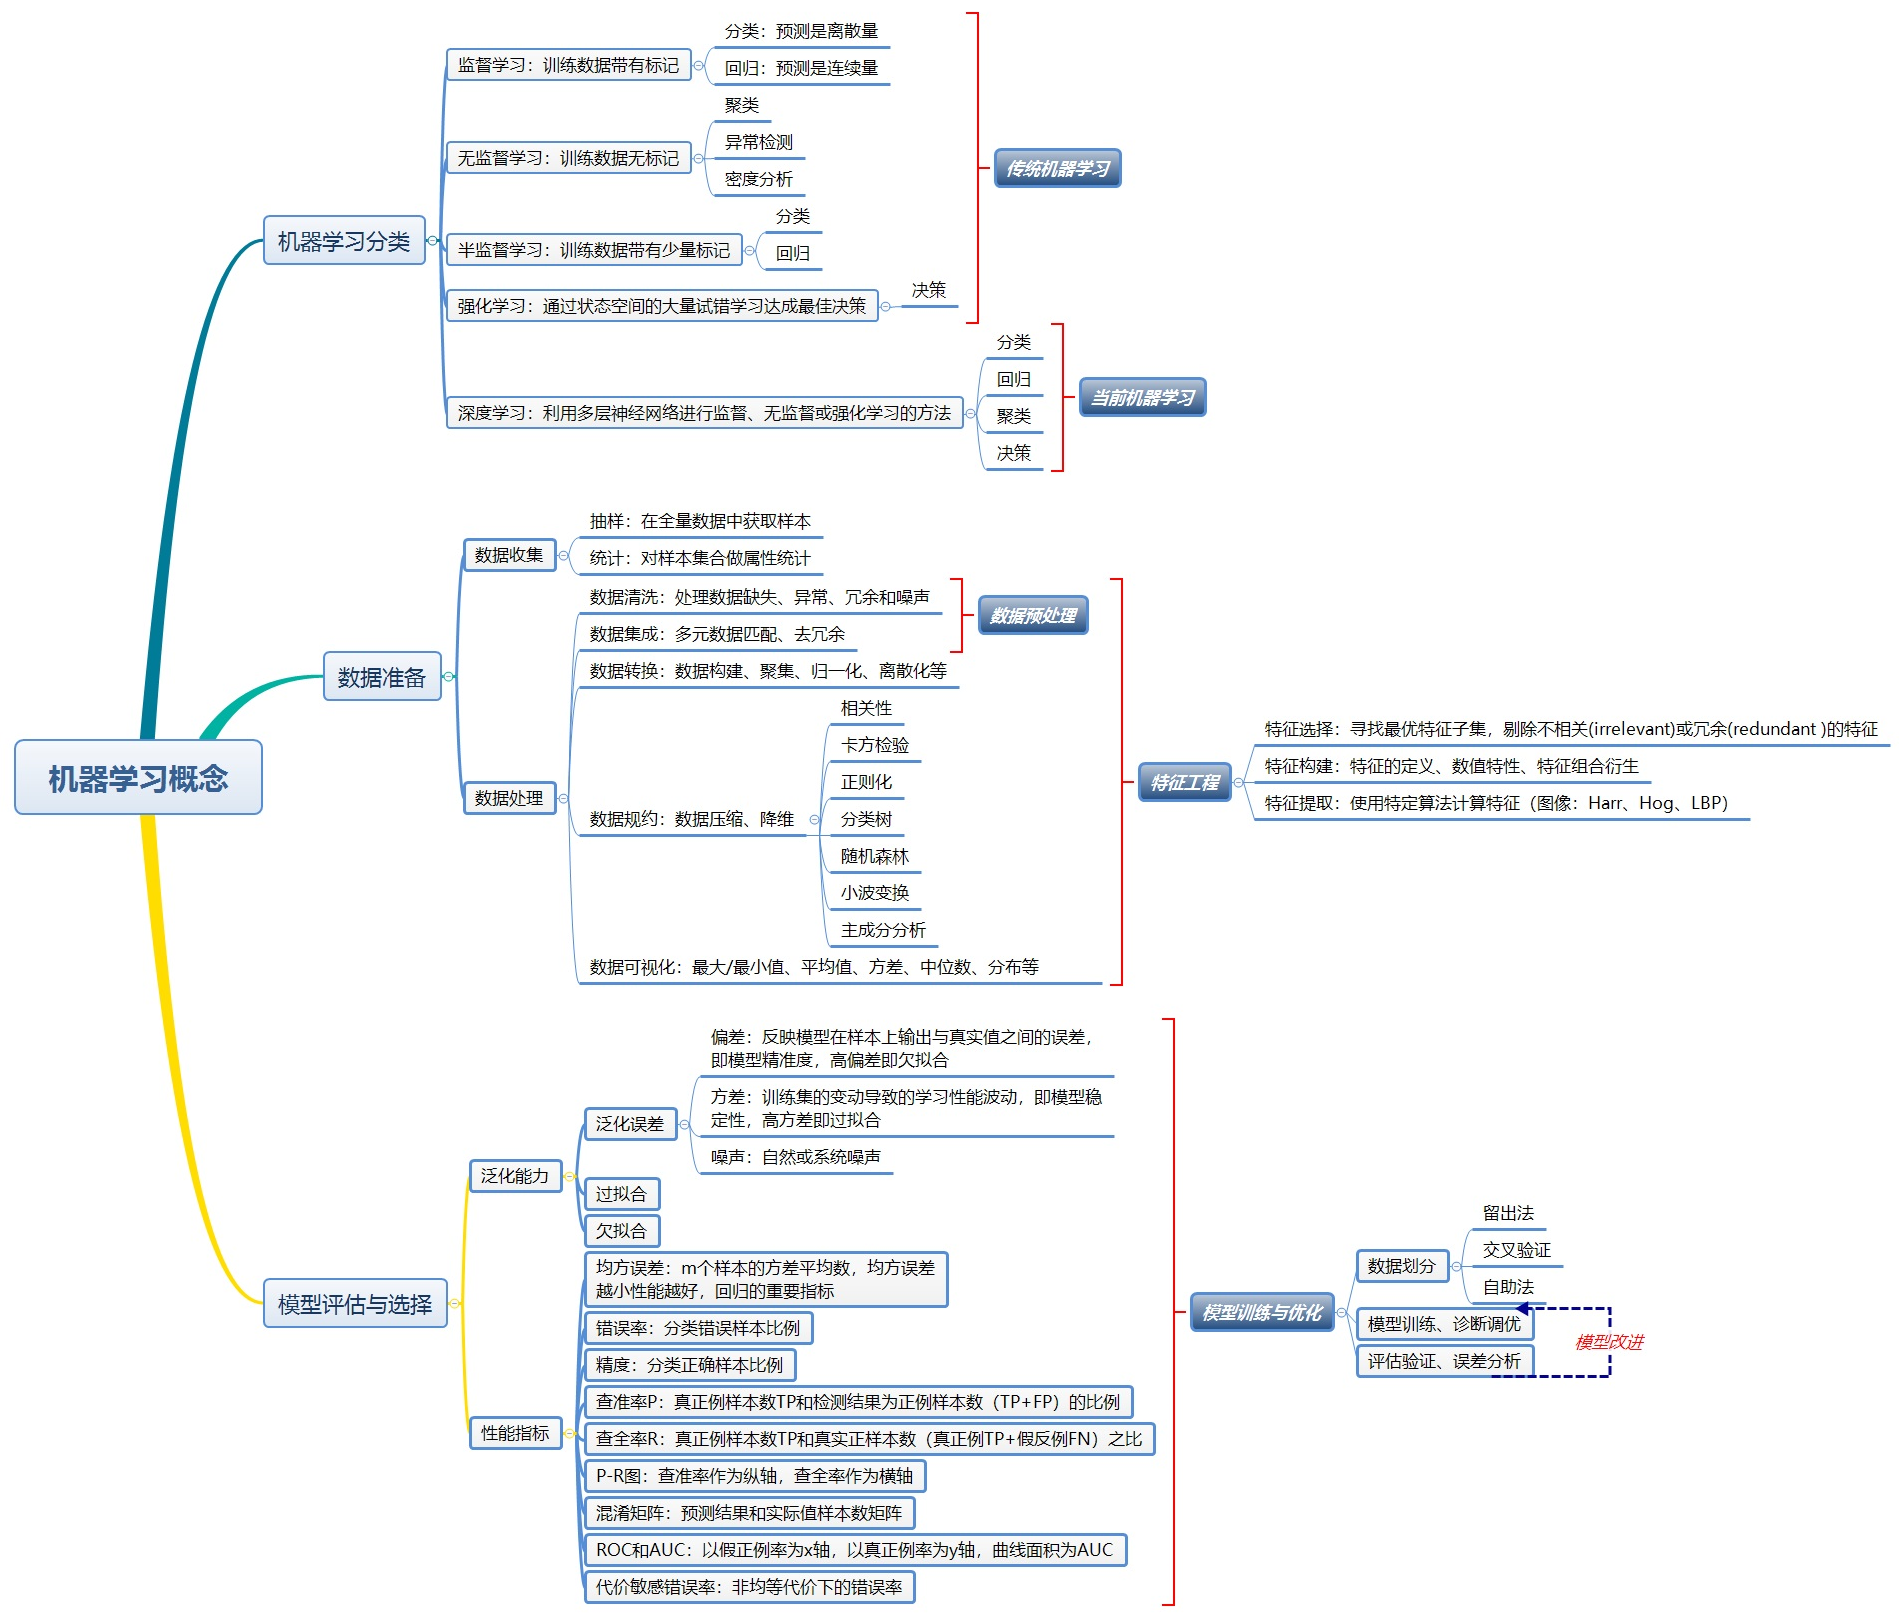
\includegraphics[width=0.7\textwidth]{image/ML-1.png}
  \caption{机器学习总知识脉络(\href{https://www.cnblogs.com/wnwin/p/9684520.html}{原图})}
\end{figure}
针对机器学习分类中各个类别所常用的模型如下图所示:
\begin{figure}[htbp]
  \centering
  \vspace{0cm}
  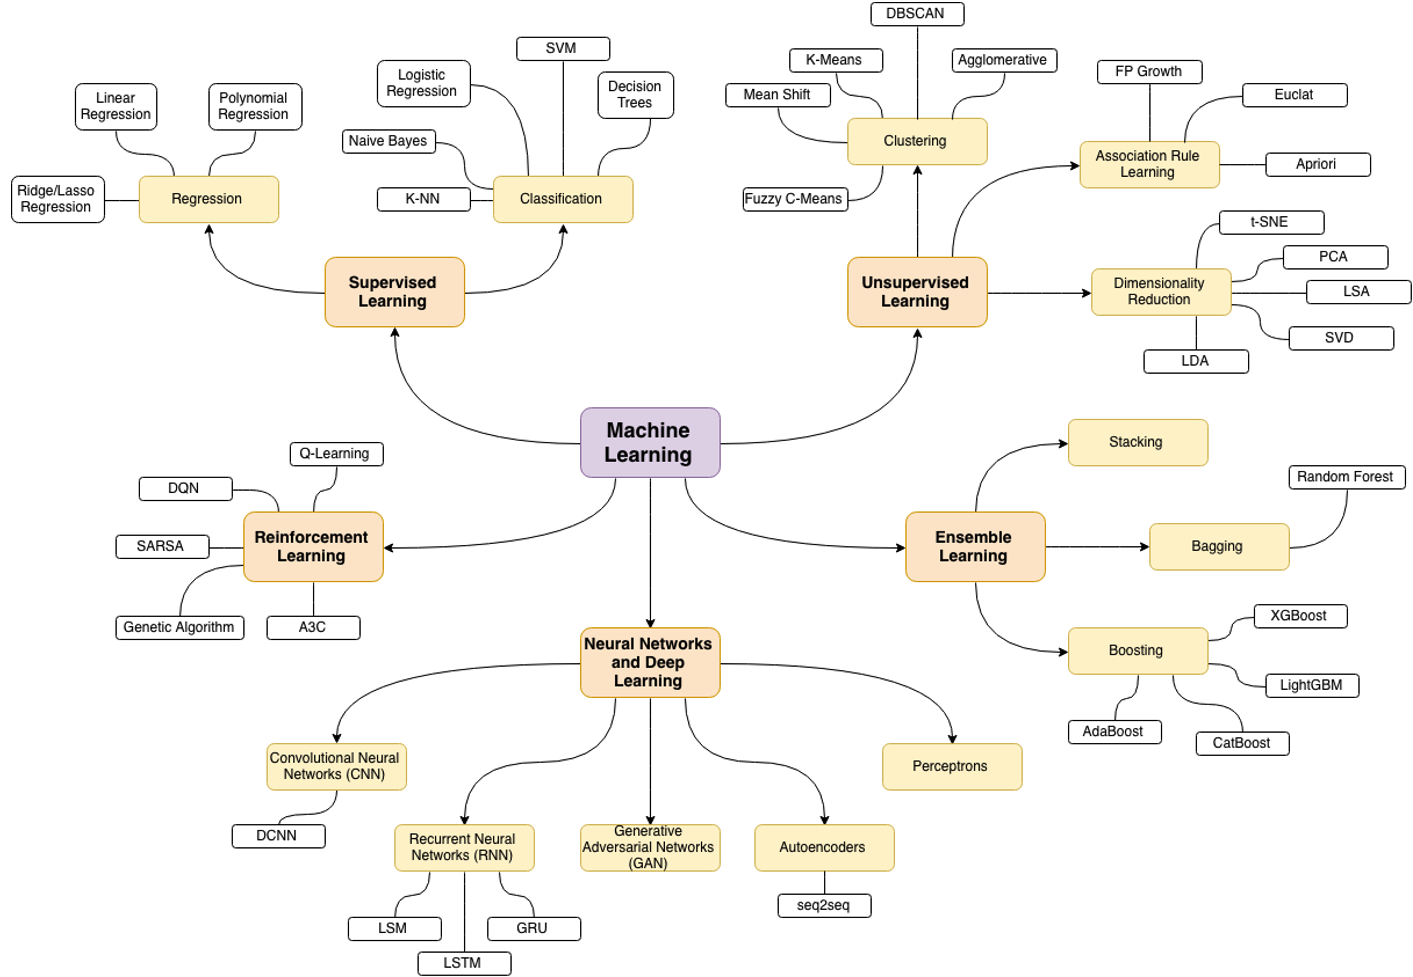
\includegraphics[width=0.7\textwidth]{image/ML-2.png}
  \caption{各个类别常用模型(\href{https://github.com/trekhleb/machine-learning-octave}{原图})}
\end{figure}

而如何分析问题并且选择模型具体如下图所示:
\begin{figure}[htbp]
  \centering
  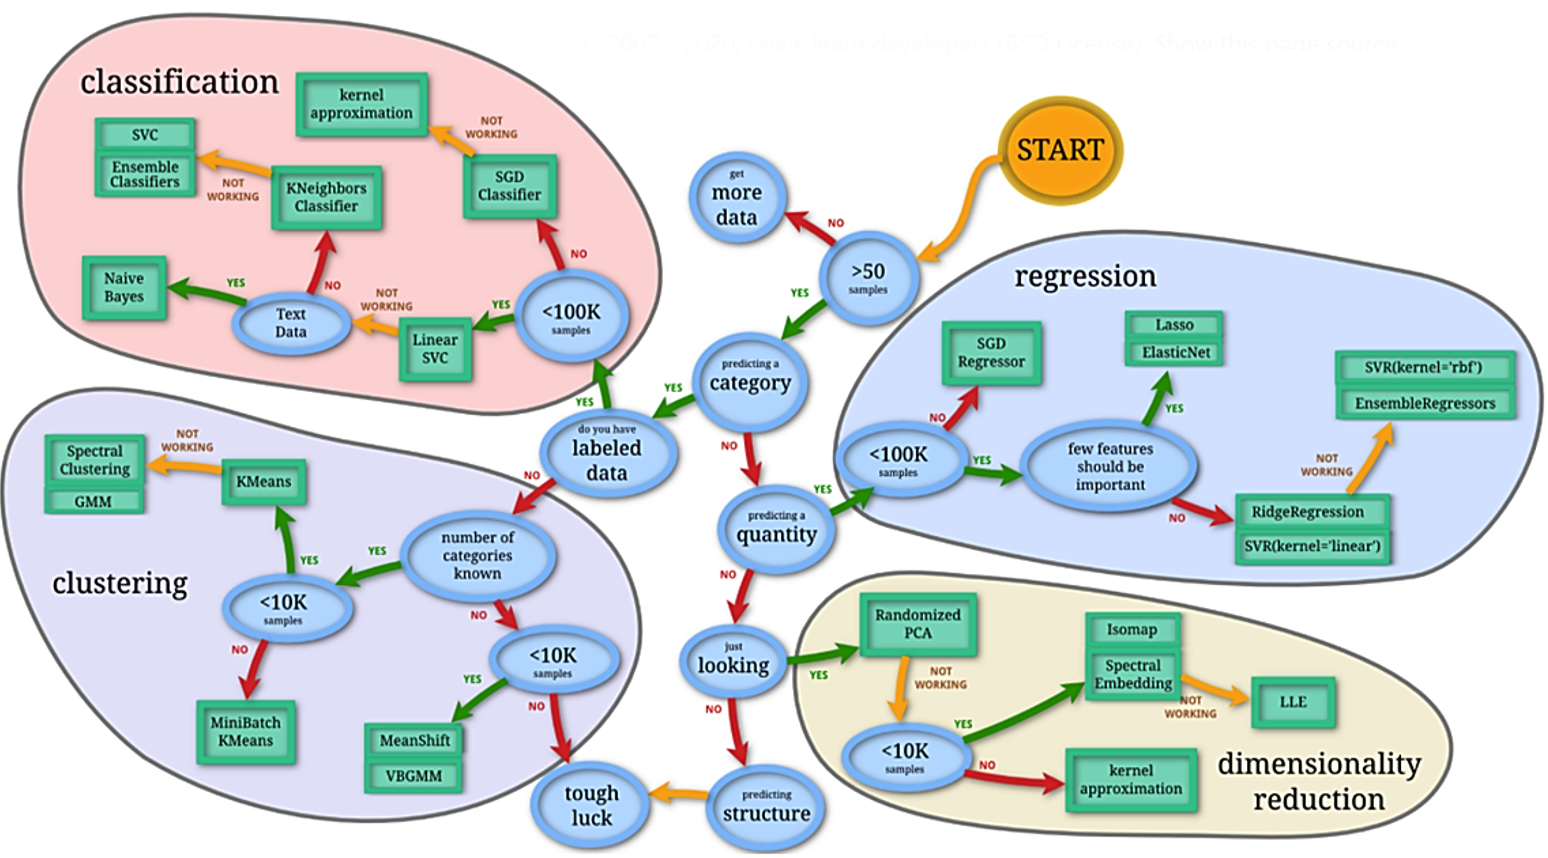
\includegraphics[width=0.7\textwidth]{image/ML-3.png}
  \caption{各类别模型选择(\href{https://scikit-learn.org/stable/tutorial/machine_learning_map/index.html}{原图})}
\end{figure}

最后推荐\href{https://whimsical.com/CA7f3ykvXpnJ9Az32vYXva}{https://whimsical.com/CA7f3ykvXpnJ9Az32vYXva},里面对于机器学习脉络有着非常详细的叙述

\subsection{学习资料}
\paragraph{书籍}
\begin{itemize}
    \item 入门:周志华的《机器学习》
    \item 公式和原理:李航的《统计学习方法》
    \item 实战:《机器学习实战》,作者是 Peter Harrington;《Python机器学习及实践 从零开始通往Kaggle竞赛之路
\end{itemize}

\paragraph{网站}
\begin{itemize}
    \item 机器学习简介:\href{https://blog.csdn.net/hohaizx/article/details/80584307}{https://blog.csdn.net/hohaizx/article/details/80584307}
    \item 机器学习十大算法:\href{https://blog.csdn.net/qq_42379006/article/details/80741808}{https://blog.csdn.net/qq\_42379006/article/details/80741808}
    \item 英文版的入门介绍,可以当课外阅读看:\href{https://machinelearningmastery.com/machine-learning-roadmap-your-self-study-guide-to-machine-learning/}{https://machinelearningmastery.com/machine-learning-roadmap-your-self-study-guide-to-machine-learning/}
    \item 人工智能、机器学习和深度学习的区别:\href{https://www.zhihu.com/question/57770020}{https://www.zhihu.com/question/57770020}
\end{itemize}

\paragraph{学习课程和ppt}
\begin{itemize}
    \item 基础版:\href{http://www.cs.cmu.edu/~tom/10701_sp11/lectures.shtml}{http://www.cs.cmu.edu/~tom/10701\_sp11/lectures.shtml} \\
课程内容:Decision Trees;Probability and Estimation;Naive Bayes;Logistic Regression;Linear Regression;Practical Issues: Feature selection etc.
    \item 进阶版:\href{http://work.caltech.edu/lectures.html}{http://work.caltech.edu/lectures.html} \\
课程内容:Theory of Generalization;The VC Dimension;Bias-Variance Tradeoff;The Linear Model II;Neural Networks;Overfitting;Regularization;Validation etc.
    \item 吴恩达机器学习:\\ \href{https://www.bilibili.com/video/BV164411b7dx}{https://www.bilibili.com/video/BV164411b7dx}
    \item 李宏毅机器学习:\\
    \href{https://www.bilibili.com/video/BV1JE411g7XF}{https://www.bilibili.com/video/BV1JE411g7XF}
\end{itemize}

\subsection{相关论文}
\begin{itemize}
    \item 线性回归:\href{https://www.researchgate.net/publication/227373853_Linear_Regression_Analysis_Theory_and_Computing_by_Xin_Yan_Xiao_Gang_Su}{Linear Regression Analysis: Theory and Computing by Xin Yan, Xiao Gang Su} 
    \item 逻辑斯蒂回归:\href{https://www.wiley.com/en-us/Applied+Logistic+Regression\%2C+3rd+Edition-p-9780470582473}{Applied logistic regression} 
    \item VC维:\href{https://dl.acm.org/doi/10.1145/76359.76371}{Learnability and the Vapnik–Chervonenkis dimension} 
    \item 支持向量机(SVM):\\
    - \href{https://dl.acm.org/doi/10.1145/130385.130401}{A training algorithm for optimal margin classifiers} \\
    - \href{https://dl.acm.org/doi/10.1023/A\%3A1022627411411}{Support vector networks}  \\
    - \href{https://www.aaai.org/Papers/KDD/1995/KDD95-030.pdf}{Extracting support data for a given task} \\
    - \href{https://dl.acm.org/doi/10.1023/A\%3A1022627411411}{Advances in Kernel Methods}
    \item K近邻算法(KNN):\href{https://citeseerx.ist.psu.edu/viewdoc/download?doi=10.1.1.1010.2854&rep=rep1&type=pdf}{An Introduction to Kernel and Nearest-Neighbor Nonparametric Regression} 
    \item 决策树与随机森林:\\
    - \href{https://onlinelibrary.wiley.com/doi/abs/10.1002/cyto.990080516}{Classification and Regression Trees} \\
    - \href{https://dl.acm.org/doi/10.1023/A\%3A1022643204877}{Induction of decision trees} \\
    - \href{https://link.springer.com/article/10.1023/A:1010933404324}{Random Forests} 
    \item Boosting:\\
    - \href{https://cseweb.ucsd.edu/~yfreund/papers/BoostByMajority.pdf}{Boosting a weak learning algorithm by majority} \\
    - \href{https://www.face-rec.org/algorithms/Boosting-Ensemble/decision-theoretic_generalization.pdf}{A decision-theoretic generalization of on-line learning and an application to boosting.} \\
    - \href{https://cseweb.ucsd.edu/~yfreund/papers/brownboost.pdf}{An adaptive version of the boost by majority algorithm} \\
    - \href{https://papers.nips.cc/paper/2017/file/6449f44a102fde848669bdd9eb6b76fa-Paper.pdf}{LightGBM: A Highly Efficient Gradient Boosting Decision Tree.} 
    \item 主成分分析(PCA):\href{https://alex.smola.org/papers/1999/MikSchSmoMuletal99.pdf}{Kernel PCA and de-noising in feature spaces}	
    \item K-means:\href{https://www.jstor.org/stable/2346830?seq=1}{A K-Means Clustering Algorithm}
    \item 神经网络:\\
    - \href{https://static1.squarespace.com/static/5b58c02775f9ee8fa7e52f00/t/5eff679acdfa560968e5f7f2/1593796507323/block_62.pdf}{The Perceptron: A Model for Brain Functioning}\\
    - \href{https://www.nature.com/articles/323533a0}{Learning representations by back-propagating errors}	\\
    - \href{http://vision.stanford.edu/cs598_spring07/papers/Lecun98.pdf}{Gradient-based learning applied to document recognition} \\
    - \href{https://ieeexplore.ieee.org/document/58337}{Backpropagation through time: what it does and how to do it} 
    \item 优化理论:\\
    - \href{https://citeseerx.ist.psu.edu/viewdoc/download?doi=10.1.1.57.5612&rep=rep1&type=pdf}{On the momentum term in gradient descent learning algorithms} \\
    - \href{https://www.microsoft.com/en-us/research/publication/stochastic-gradient-tricks/}{Stochastic Gradient Descent Tricks.}	\\
    - \href{https://arxiv.org/abs/1412.6980}{Adam: a method for stochastic optimization}
\end{itemize}

\section{计算机视觉}
\subsection{传统算法的识别和跟踪}
\begin{figure}[htbp]
  \centering
  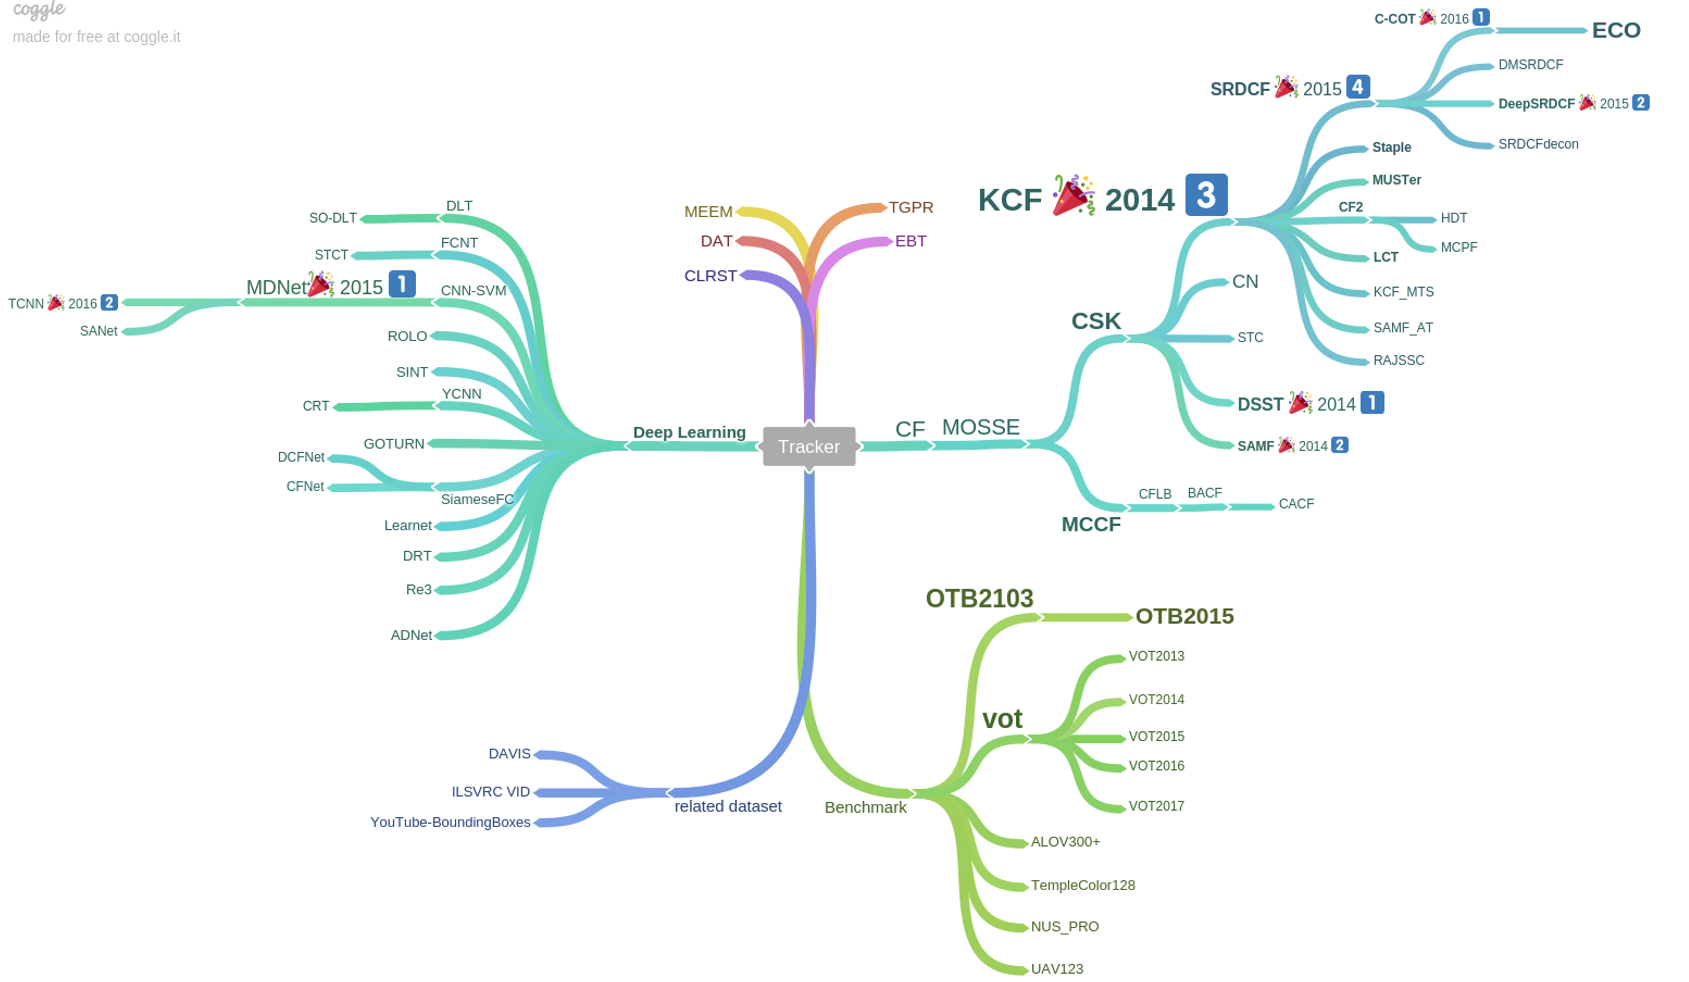
\includegraphics[width=0.9\textwidth]{image/cv_1.png}
  \caption{传统识别跟踪算法的知识脉络图}
\end{figure}

对图片或者视频内容的识别和跟踪是一个相当普遍的任务,发展时间很长,历经了从传统方法到机器学习方法的转变,但是在小型无人机或者无人车等计算资源有限的环境下,一般还是考虑采取传统的方法。传统方法里应该就是两个最有代表性的算法,\textbf{TLD}和\textbf{KCF}。

\paragraph{TLD} TLD叫Tracking-Learning-Detection,主要由追踪器(Tracker)、检测器(Detector)和学习(Learning)三个模块构成。TLD是对视频中未知物体的长时间跟踪的算法,未知物体指的是任意的物体,在开始追踪之前不知道哪个物体是目标。物体始终可见时使用追踪器连续跟踪,检测器对图像进行全面扫描更新追踪器的初始位置,学习器迭代训练分类器,改善检测器的精度。

\paragraph{KCF} 第二个最有代表的算法就是KCF,kernel correlation filter,核相关滤波算法,其核心思想是设计一个滤波的模板,使得这个模板作用在整张图片上时,作用到跟踪目标上得到的响应最大,在背景上响应较小。而这个滤波模板则能够通过正负样本的循环采取和岭回归进行不断训练,从而对目标进行长时间的跟踪。
 
\hfill 
 
总的来说,传统方法是从对图像的理解上出发,基于严格的数学推导去识别和跟踪视频中移动的物体,涉及图像的傅立叶变换,线性与非线性回归,和相当多的机器学习(不是深度学习)知识。在后人不断改进下,应用范围也不断增广,如DS-KCF,能用于在深度图上进行跟踪,鲁棒性与实时性也不断提高,在机器人领域有着广泛的应用价值。

之后深度学习开始火起来,使用卷积神经网络的图像检测与跟踪算法层出不穷,像大名鼎鼎、不断迭代更新的yolo系列,但是基于学习的方法一是需要大量样本训练,二是泛化性不高,三是对设备的要求较高,因此基于自监督的方法越来越受到人们的关注,个人没有很积极关注,有兴趣的同学可以好好研究。

上面提到的经典论文:
\begin{itemize}
    \item TLD:\href{http://vision.stanford.edu/teaching/cs231b_spring1415/papers/Kalal-PAMI.pdf}{http://vision.stanford.edu/teaching/cs231b\_spring1415/papers/Kalal-PAMI.pdf}
    \item KCF:\href{https://arxiv.org/pdf/1404.7584}{https://arxiv.org/pdf/1404.7584}
    \item DS-KCF:\href{https://pdfs.semanticscholar.org/3aa4/573f8735e984c25db8b2a805235bf22dc042.pdf}{https://pdfs.semanticscholar.org/3aa4/573f8735e984c25db8b2a805235bf22dc042.pdf}
\end{itemize}

\paragraph{相关的网课与书籍} 
\begin{itemize}
    \item 数字图像处理(冈萨雷斯版)  大部头书籍,很难啃,一般当百科全书用。
    \item 斯坦福大学CS231n: \href{http://cs231n.stanford.edu/syllabus.html}{Convolutional Neural Networks for Visual Recognition}。经典CS231n,主要涉及深度学习方法。
    \item 普林斯顿大学的tracking的benchmark: \href{http://tracking.cs.princeton.edu/}{http://tracking.cs.princeton.edu/}
\end{itemize}

\subsection{目标检测}
\begin{figure}[htbp]
  \centering
  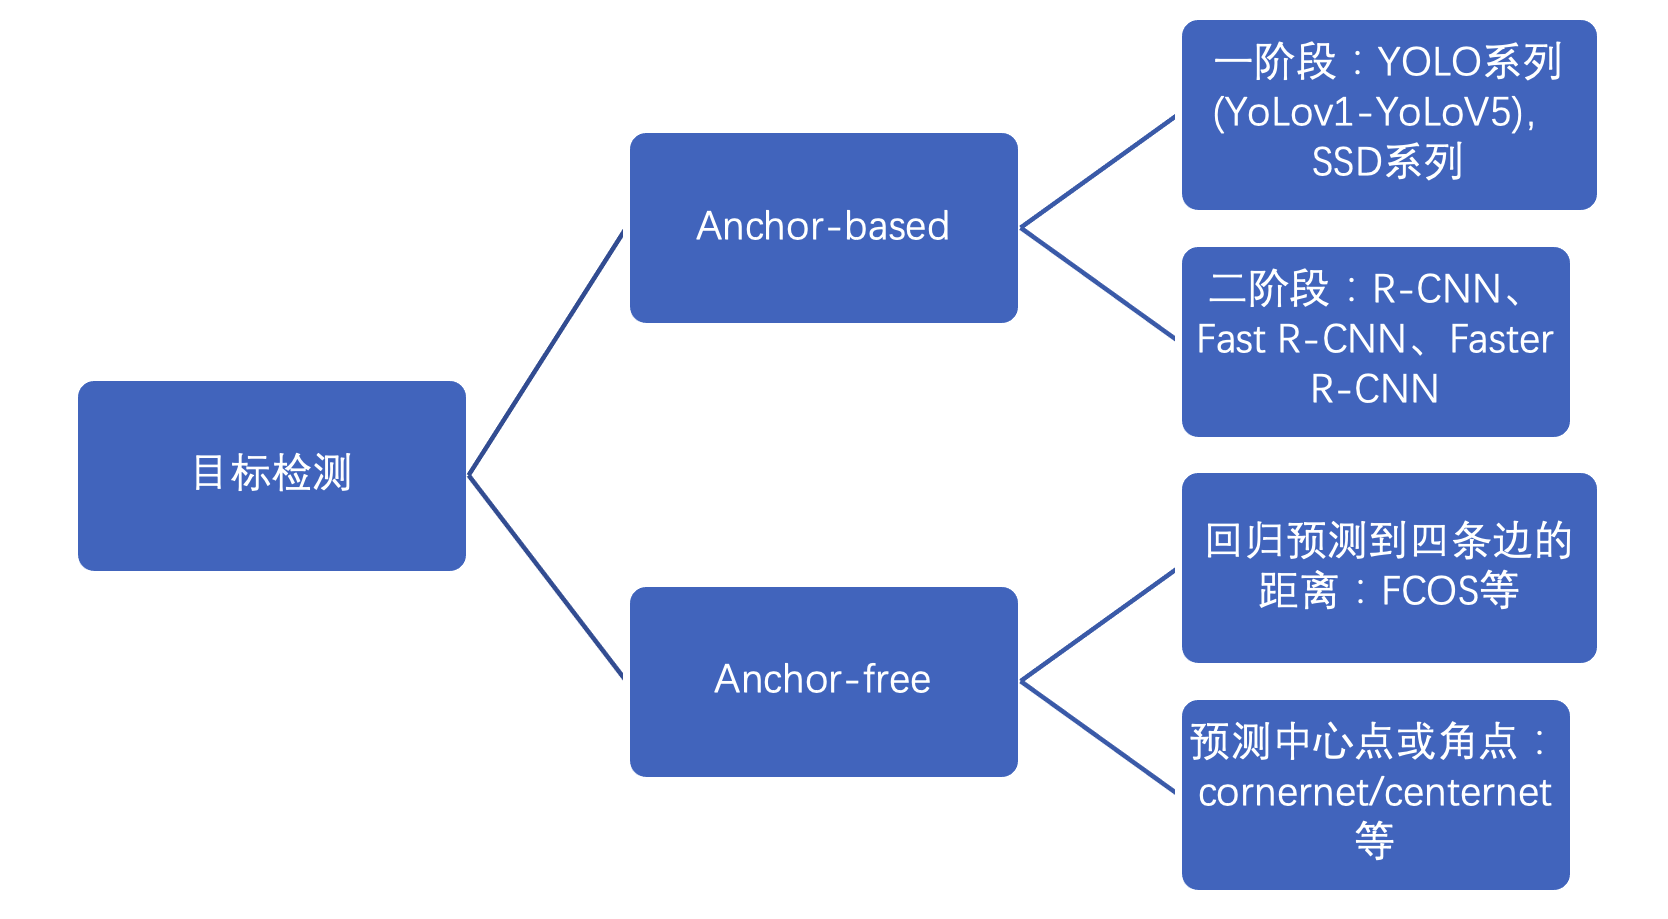
\includegraphics[width=0.8\textwidth]{image/cv_2.png}
  \caption{目标检测知识脉络图}
\end{figure}

\begin{figure}[htbp]
  \centering
  \vspace*{-3cm}
  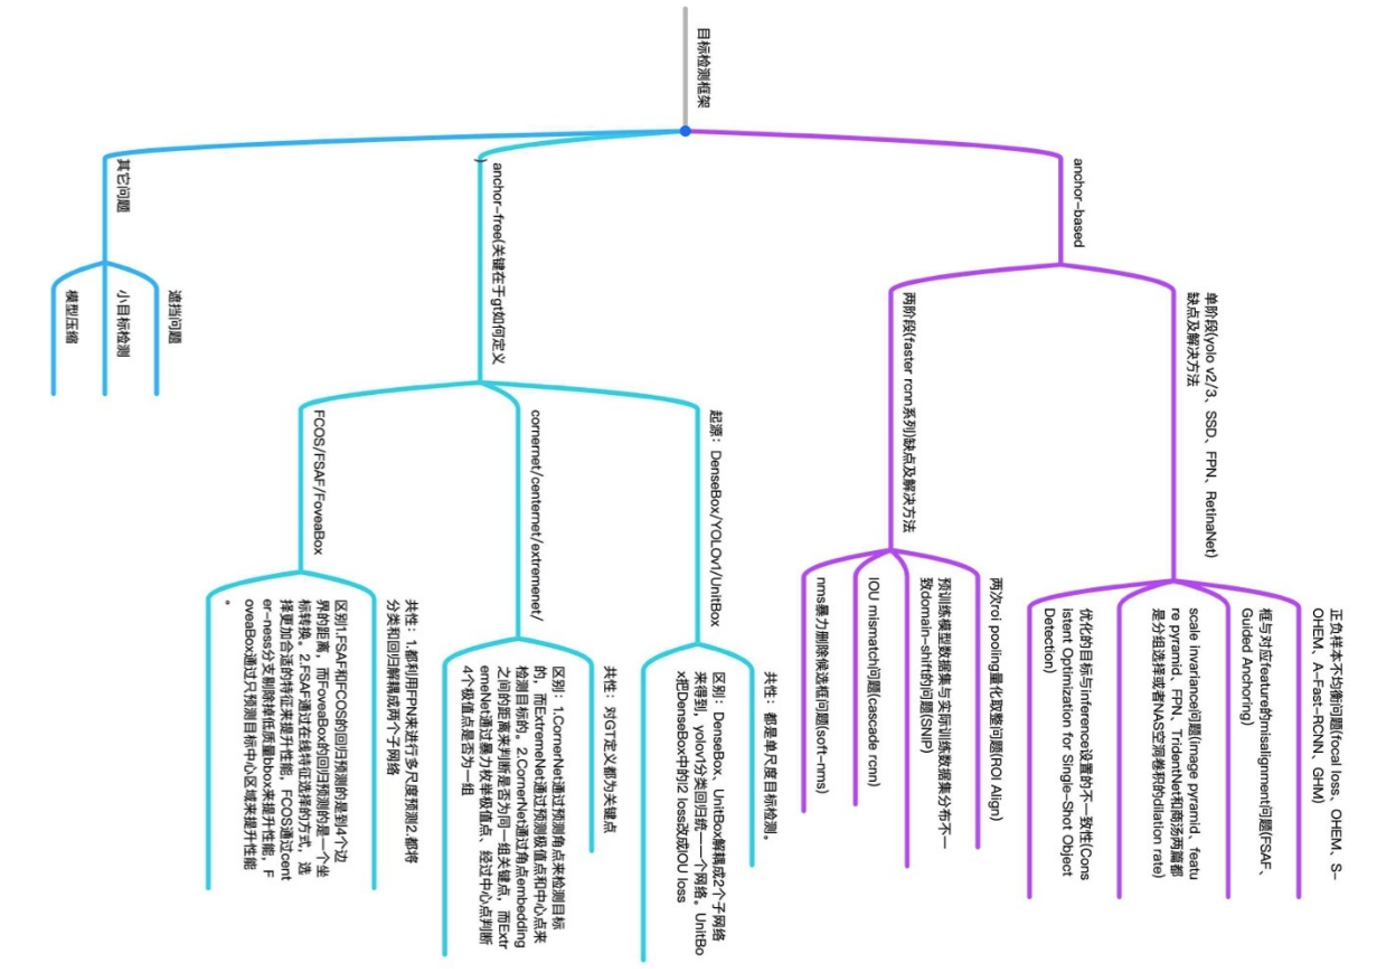
\includegraphics[scale=0.3, angle=90]{image/cv_3.png}
  \caption{目标检测详细知识脉络图}
\end{figure}

\begin{figure}[htbp]
  \centering
  \vspace*{-4cm}
  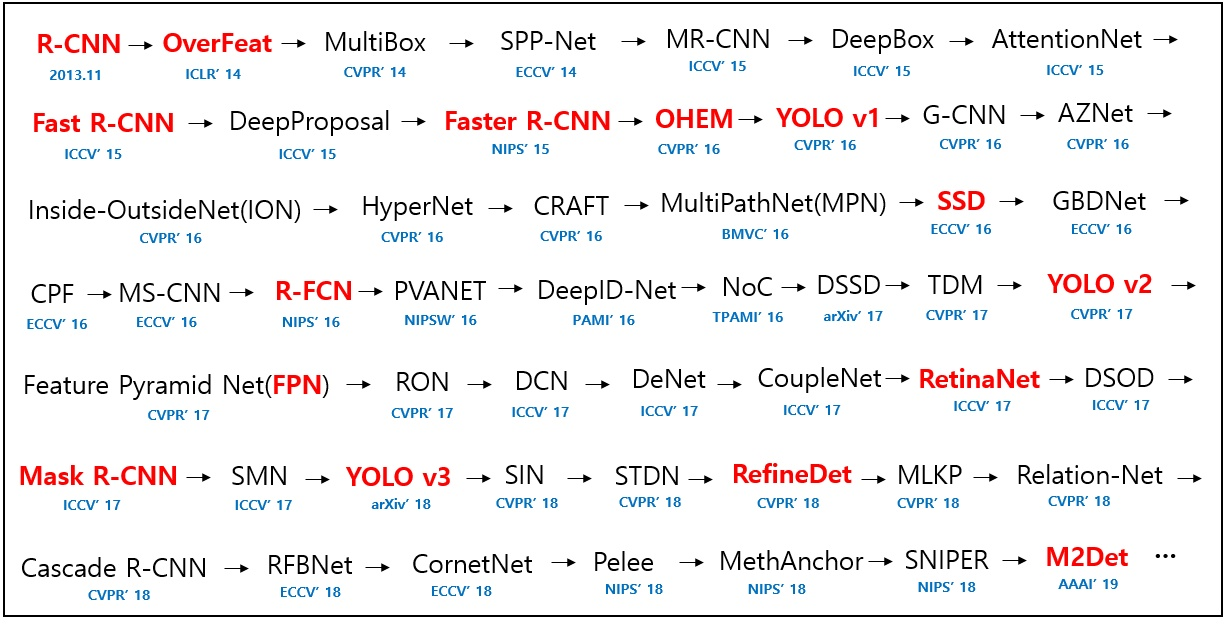
\includegraphics[scale=0.35]{image/cv_4.jpg}
  \caption{目标检测算法发展时间线}
\end{figure}

性能对比汇总表(评价指标mAP):
\begin{figure}[htbp]
  \centering
  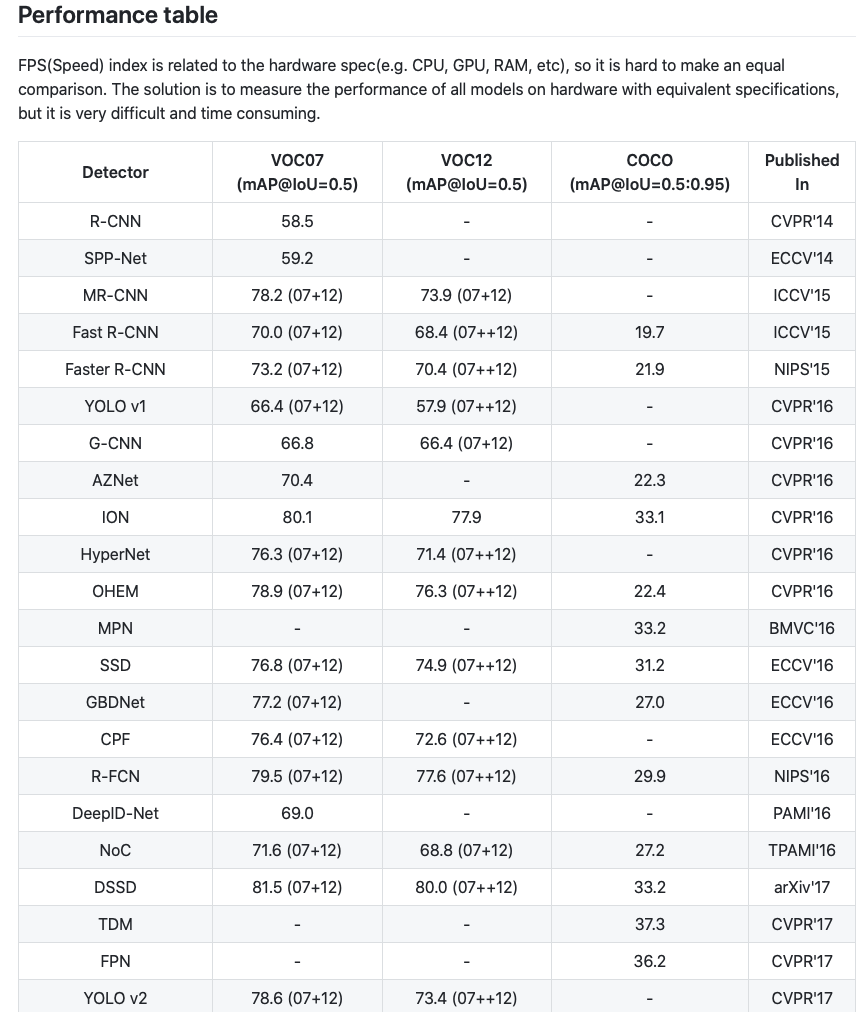
\includegraphics[width=0.85\textwidth]{image/cv_5.png}
  \caption{检测算法benchmark}
\end{figure}

\hfill 

经典论文:\href{https://github.com/hoya012/deep_learning_object_detection}{https://github.com/hoya012/deep\_learning\_object\_detection}
看这个链接就够了,从2014-2020按照时间线,列举了有重大贡献的论文和其开源代码。

\hfill 

其他网课,书籍,资料(经典的Review/Survey)推荐:\\
1.	公开课:斯坦福大学CS231n: Convolutional Neural Networks for Visual Recognition\\
链接:\href{http://cs231n.stanford.edu/syllabus.html}{http://cs231n.stanford.edu/syllabus.html}\\
2.	吴恩达 深度学习第4篇 计算机视觉(3.9目标检测)\\
链接:\href{https://www.bilibili.com/video/BV1gb411j7Bs?from=search&seid=722731644245107858}{https://www.bilibili.com/video/BV1gb411j7Bs?from=search\&seid=722731644245107858}\\
3.	天池-目标检测 \href{https://tianchi.aliyun.com/course/video?liveId=41141}{https://tianchi.aliyun.com/course/video?liveId=41141}

\subsection{目标追踪}
现有的目标追踪主要分为两个任务方向,即单目标追踪(single object tracking,SOT)与多目标追踪(multi object tracking)。主要针对的对象是行人、车辆。
\begin{figure}[htbp]
  \centering
  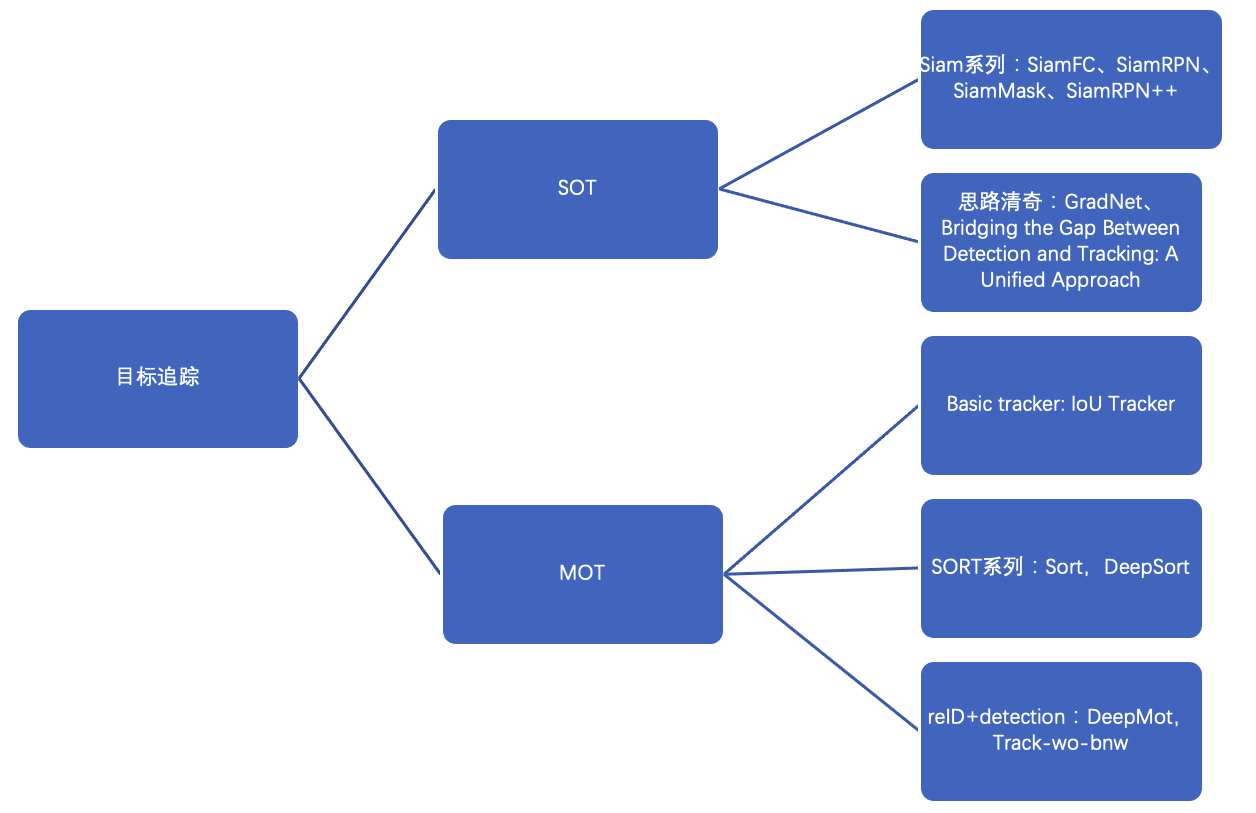
\includegraphics[width=0.75\textwidth]{image/cv_6.png}
  \caption{目标追踪知识脉络}
\end{figure}
p.s. MOT部分,自DeepSort之后,大家慢慢把多目标追踪改造成一个reid和detection的联合任务(用于解决工程情况下容易出现的长时间遮挡情况)

\hfill
\paragraph{经典论文}
\begin{enumerate}
    \item SiamFC:\\
    论文地址:\href{https://arxiv.org/pdf/1606.09549.pdf}{https://arxiv.org/pdf/1606.09549.pdf}(ECCV 2016) \\
    代码:\href{https://github.com/torrvision/siamfc-tf}{https://github.com/torrvision/siamfc-tf}  \\
    主要贡献:单目标追踪siamese系列的开山之作,目前大半的SOT任务都使用siamese网络完成,主要的思路是将跟踪当作匹配问题,帮助模型高效精确定位
    \item GradNe:\\
    论文地址:\href{https://arxiv.org/pdf/1909.06800.pdf}{https://arxiv.org/pdf/1909.06800.pdf}(ICCV 2019) \\
    代码:\href{https://github.com/LPXTT/GradNet-Tensorflow}{https://github.com/LPXTT/GradNet-Tensorflow}  \\
    主要贡献:针对Siam系列网络不实时更新背景信息的问题,使用在线BP熏蒸template,帮助模型学习背景信息,提升模型的精度。
    \item IoU Tracker:\\
    论文地址:\href{http://elvera.nue.tu-berlin.de/files/1517Bochinski2017.pdf}{http://elvera.nue.tu-berlin.de/files/1517Bochinski2017.pdf}(AVSS 2017) \\
    代码:\href{https://github.com/bochinski/iou-tracker}{https://github.com/bochinski/iou-tracker}(非官方复现) \\
    主要贡献:提出了一种简单高效的跟踪模型——IOU Tracker。速度快、基于TBD(tracking-by-detection)、不需要图像信息。
    \item Sort:\\
    论文地址:\href{https://arxiv.org/pdf/1602.00763.pdf}{https://arxiv.org/pdf/1602.00763.pdf}(ICIP 2017) \\
    代码:\href{https://github.com/abewley/sort}{https://github.com/abewley/sort} \\
    主要贡献:引入kalman滤波预测目标状态,结合检测框位置和IOU的匈牙利算法进行检测框的匹配,提升算法精度,且检测较为高效。
    \item DeepSort:
    论文地址:\href{https://arxiv.org/pdf/1703.07402.pdf}{https://arxiv.org/pdf/1703.07402.pdf}(WACV 2018)\\
    代码:\href{https://github.com/nwojke/deep_sort}{https://github.com/nwojke/deep\_sort} \\
    主要贡献:在匹配阶段引入马氏距离和表观匹配(reid),结合运动和图像信息减少了预测时出现的ID switch。
    \item Tracking without bells and whistles:\\ 
    论文地址:\href{https://arxiv.org/pdf/1903.05625.pdf}{https://arxiv.org/pdf/1903.05625.pdf}(ICCV 2019) \\
    代码:\href{https://github.com/phil-bergmann/tracking_wo_bnw}{https://github.com/phil-bergmann/tracking\_wo\_bnw}  \\
    主要贡献:作提出将目标检测器转换为追踪器,不特意去对当前存在的遮挡,重识别和运动预测进行优化而完成跟踪任务。且不需要进行训练和优化。利用对象检测器的边界框回归来预测对象在下一帧中的新位置,通过简单的重新识别和相机运动补偿对其进行扩展, 展示了跟踪器的可扩展。
\end{enumerate}

\paragraph{目标追踪数据集/比赛/benchmark} 
\begin{itemize}
\item \href{http://www.cvg.reading.ac.uk/PETS2009/a.html}{PETS2009} : An old dataset.
\item \href{https://motchallenge.net/}{MOT dataset} : A dataset for multi-person detection and tracking, mostly used.
\item \href{http://detrac-db.rit.albany.edu/}{UA-DETRAC} : A dataset for multi-car detection and tracking. 
\item \href{https://iwt4s2018.wordpress.com/challenge/}{AVSS2018 Challenge} : AVSS2018 Challenge based on UA-DETRAC is opened!
\item \href{http://vision.cs.duke.edu/DukeMTMC/}{DukeMTMC} : A dataset for multi-camera multi-person tracking. 
\item \href{https://posetrack.net/}{PoseTrack}: A dataset for multi-person pose tracking. 
\item \href{https://www.aicitychallenge.org/}{NVIDIA AI CITY Challenge}: Challenges including "Traffic Flow Analysis", "Anomaly Detection" and "Multi-sensor Vehicle Detection and Reidentification", you may find some insteresting codes on their Github repos
\item \href{http://www.aiskyeye.com/views/index}{Vis Drone}: Tracking videos captured by drone-mounted cameras.
\item \href{http://imagelab.ing.unimore.it/imagelab/page.asp?IdPage=25}{JTA Dataset}: A huge dataset for pedestrian pose estimation and tracking in urban scenarios created by exploiting the highly photorealistic video game Grand Theft Auto V developed by Rockstar North.
\item \href{http://people.ee.ethz.ch/~daid/pathtrack/}{Path Track}: A new dataset with many scenes.
\item \href{https://www.vision.rwth-aachen.de/page/mots}{MOTS MOTS}: Multi-Object Tracking and Segmentation. In CVPR 2019
\end{itemize}


\paragraph{Reference} 
\begin{enumerate}[label={[\arabic*]}, noitemsep]
\item \href{https://github.com/SpyderXu/multi-object-tracking-paper-list}{https://github.com/SpyderXu/multi-object-tracking-paper-list} 
\item \href{https://zhuanlan.zhihu.com/p/65177442}{https://zhuanlan.zhihu.com/p/65177442} 
\item \href{https://link.zhihu.com/?target=https\%3A//github.com/huanglianghua/mot-papers/blob/master/README.md}{https://link.zhihu.com/?target=https\%3A//github.com/huanglianghua/mot-papers/blob/master/README.md} 
\end{enumerate}

\subsection{图像分割}
\begin{figure}[htbp]
  \centering
  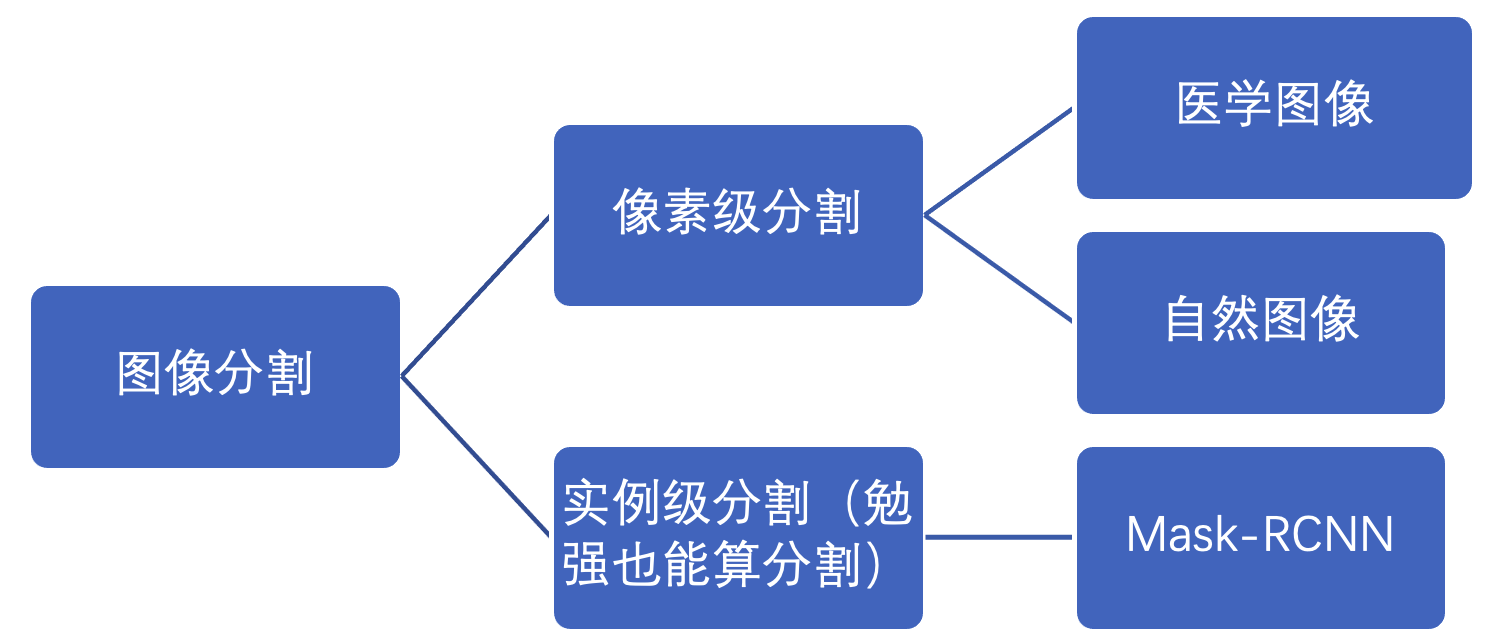
\includegraphics[width=0.8\textwidth]{image/cv_7.png}
  \caption{图像分割主要知识脉络(其实主要就是像素级分割)}
\end{figure}
分割是个很普遍存在的任务,相关的东西很多很杂乱,所以没有发展脉络图。下面主要说一下几个里程碑。

深度学习火起来之前像素级分割是很难的任务,但是后来卷积在AlexNet上大放异彩后迅速被用到了分割上,于是现在分割可以算是一个比较简单的东西了。实际上,像素级的分割无非就是对每个像素做分类,所以在很多时候损失函数依然可以沿用分类任务里常见的交叉熵损失函数。至今,分割依然保持着和分类任务极为相近的思路,都是先用卷积提取特征,只不过分类任务是后面接全连接,而分割后面是接卷积和上采样等等操作罢了。

这种把全连接换成卷积的网络就是全卷积网络,这是第一个里程碑,也是语义分割的开山之作。

\hfill

如果硬要说第二个里程碑的话,那可能就是空洞卷积和特征金字塔,这些都是Deeplab系列网络提出来的新概念。其中空洞卷积就是在普通卷积核中间插入孔洞,使其感受野(就是它一次计算能覆盖的像素范围)增大同时参数量不变;金字塔池化就是多个卷积层叠呈金字塔形,并且允许一层存在多个不同大小和形式的卷积核,只要在最后将卷积核的输出结果合并到一起就好了。不过这个东西实际用起来效果并不是那么稳定的,我个人感觉算不上里程碑吧,但现在只要是相关的课程都会讲。

我个人认为的一个非常重要的里程碑是UNet的诞生。该网络本来是用于医学图像分割的,但是经过千锤百炼证明了自己在自然图像上照样管用,超分辨也经常用它。这个网络极为鲁棒、通用性高、结构也相对简单,强烈推荐大家干什么都可以用它试试。Unet本身是Encoder-Decoder的设计,但是在Encoder和Decoder之间采用了跨层连接的设计,这样网络能够很好地融合低维特征和高维特征,非常适合医学图像里的一些类似肿瘤分割的任务。

\begin{figure}[htbp]
  \centering
  
\includegraphics[width=0.8\textwidth]{image/cv_8.png}
  \caption{图像分割算法发展时间线}
\end{figure}

\paragraph{上面提到的经典论文}
\begin{itemize}
    \item FCN \\
    论文地址:\href{https://arxiv.org/abs/1411.4038}{https://arxiv.org/abs/1411.4038} 
    \item Deeplab系列以最新的Deeplab v3+为例(实际上也是好几年前了)\\
    论文地址:\href{https://arxiv.org/pdf/1802.02611.pdf}{https://arxiv.org/pdf/1802.02611.pdf} \\
    代码地址:\href{https://github.com/tensorflow/models/tree/master/research/deeplab}{https://github.com/tensorflow/models/tree/master/research/deeplab} 
    \item UNet \\
    论文地址:\href{https://arxiv.org/pdf/1505.04597.pdf}{https://arxiv.org/pdf/1505.04597.pdf} \\
    代码地址:\href{https://github.com/jakeret/tf_unet}{https://github.com/jakeret/tf\_unet} 
\end{itemize}
另外,可以用一些如VOC,Cityscapes之类的数据集跑一下就知道是什么个情况了。

\section{自然语言处理}
\begin{figure}[htbp]
  \centering
  \vspace{0cm}
  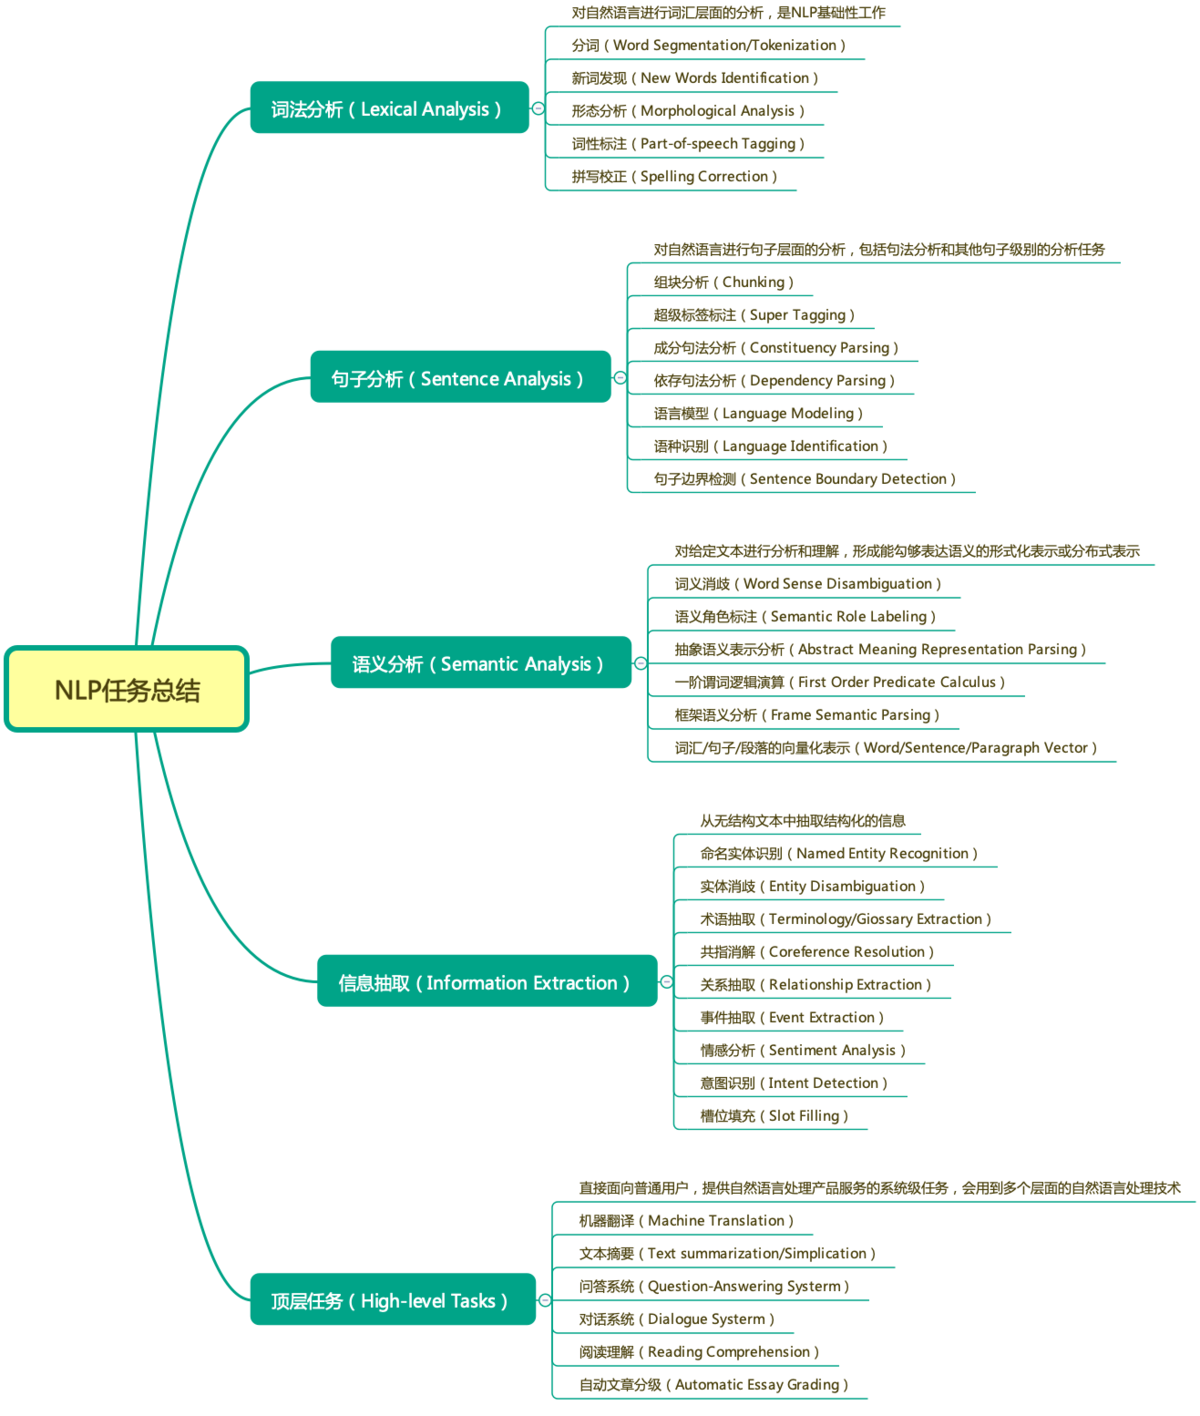
\includegraphics[width=0.8\textwidth]{image/nlp_1.png}
  \caption{自然语言处理任务分类以及子领域(\href{https://www.jianshu.com/p/d80b065bdcf0}{原图})}
\end{figure}

\begin{figure}[htbp]
  \centering
  \vspace{-2cm}
  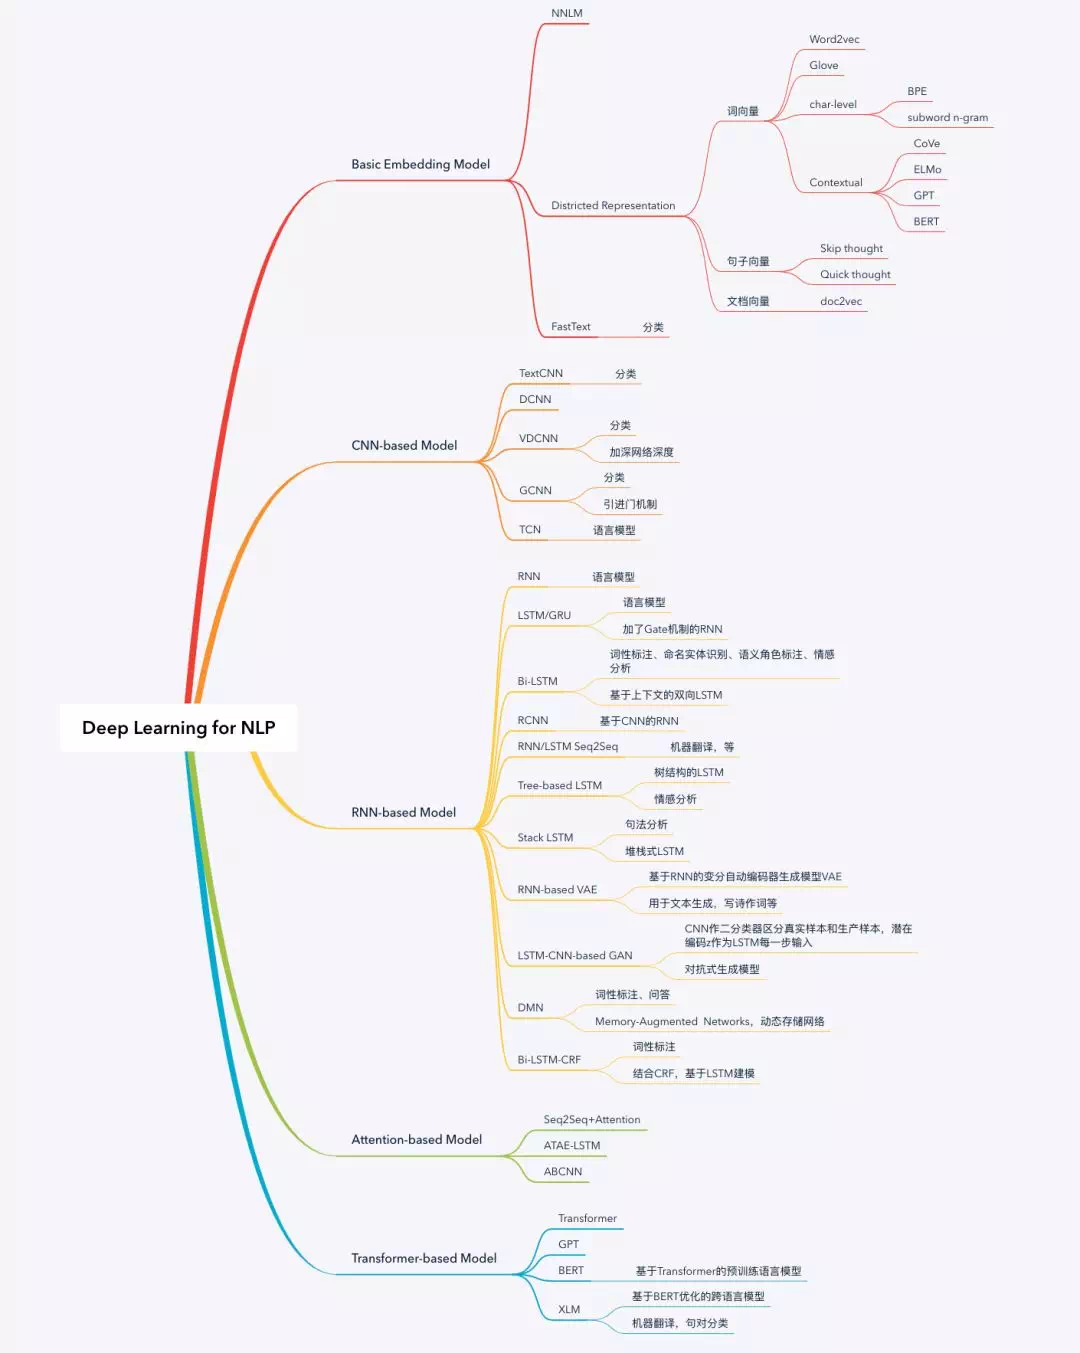
\includegraphics[width=0.8\textwidth]{image/nlp_2.png}
  \caption{自然语言处理知识脉络图(\href{https://www.jiqizhixin.com/articles/2019-06-21}{原图})}
\end{figure}

\begin{figure}[htbp]
  \centering
  \vspace{-1cm}
  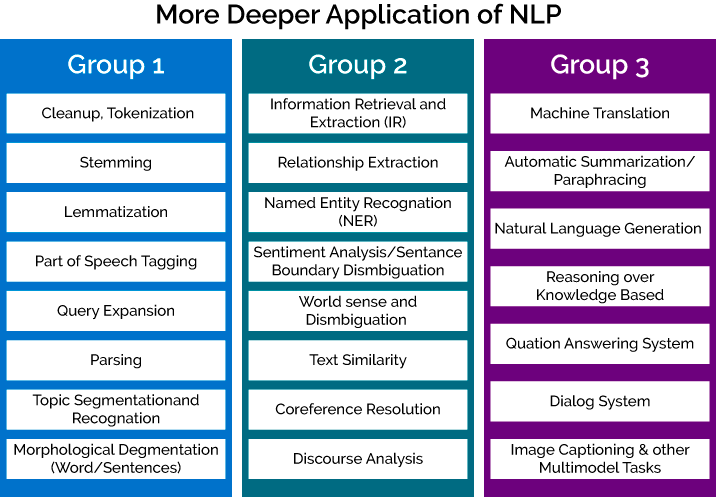
\includegraphics[width=0.6\textwidth]{image/nlp_3.png}
  \caption{Group1到Group3:底层/基础任务到顶层/具体应用(\href{https://www.packtpub.com/product/python-natural-language-processing/9781787121423}{原图})}
\end{figure}

\begin{figure}[htbp]
  \centering
  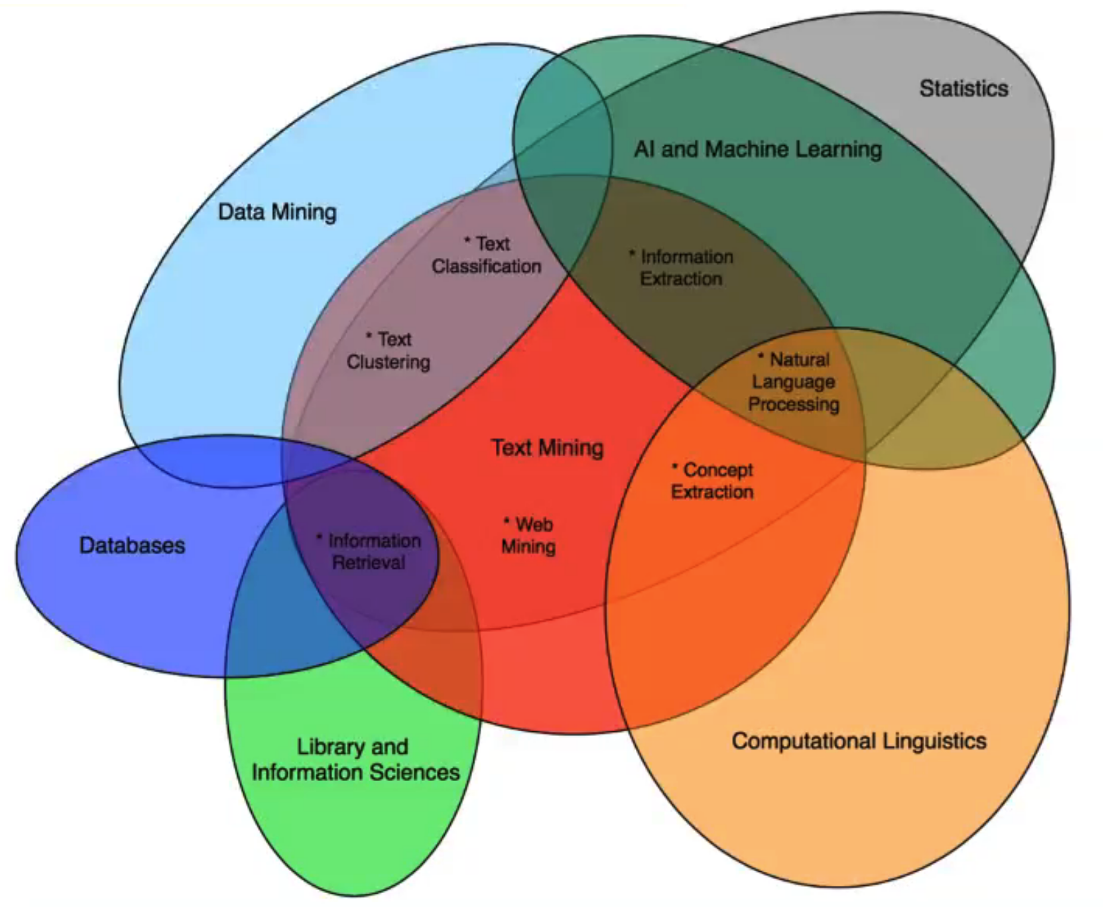
\includegraphics[width=0.7\textwidth]{image/nlp_4.png}
  \caption{自然语言处理任务子领域之间的交叉关系。\href{https://bbds.ma/wp-content/uploads/2017/11/BBDS-Deep-Learning-NLP-Text-Mining-2.pdf}{原图}}
\end{figure}

\subsection{经典论文}
\begin{enumerate}
    \item Seq2Seq + Attention\\
    论文:\href{https://papers.nips.cc/paper/5346-sequence-to-sequence-learning-with-neural-networks.pdf}{https://papers.nips.cc/paper/5346-sequence-to-sequence-learning-with-neural-networks.pdf}  \\
    实现:\href{https://github.com/google/seq2seq}{https://github.com/google/seq2seq}  \\
    贡献:Seq2Seq模型与注意力机制的结合。 
    \item Transformer\\
    论文:\href{https://arxiv.org/pdf/1706.03762.pdf}{https://arxiv.org/pdf/1706.03762.pdf}  \\
    tf实现:\href{https://github.com/Kyubyong/transformer}{https://github.com/Kyubyong/transformer} \\
    pytorch实现:\href{https://github.com/jadore801120/attention-is-all-you-need-pytorch}{https://github.com/jadore801120/attention-is-all-you-need-pytorch}  \\
    贡献:用全attention的结构代替了lstm,在翻译任务上取得了更好的成绩。Transformer改进了RNN最被人诟病的训练慢的缺点,利用self-attention机制实现快速并行。并且Transformer可以增加到非常深的深度。
    \item ELMo\\
    论文:\href{https://arxiv.org/pdf/1802.05365.pdf}{https://arxiv.org/pdf/1802.05365.pdf}  \\
    贡献:根据当前上下文对Word Embedding动态调整,而非过去的静态词嵌入。
    \item BERT \\
    论文:\href{https://arxiv.org/abs/1810.04805}{https://arxiv.org/abs/1810.04805}  \\
    tensorflow实现:\href{https://github.com/google-research/bert}{https://github.com/google-research/bert} \\
    pytorch实现:\href{https://github.com/huggingface/transformers}{https://github.com/huggingface/transformers}  \\
    贡献:1)使用了Transformer作为算法的主要框架,Transformer能更彻底的捕捉语句中的双向关系;\\
    2)使用了Mask Language Model(MLM)和 Next Sentence Prediction(NSP) 的多任务训练目标;\\
    3)使用更强大的机器训练更大规模的数据,使BERT的结果达到了全新的高度,并且Google开源了BERT模型,用户可以直接使用BERT作为Word2Vec的转换矩阵并高效的将其应用到自己的任务中。
    \item XLM \\
    论文:\href{https://arxiv.org/abs/1901.07291}{https://arxiv.org/abs/1901.07291}  \\
    实现:\href{https://github.com/facebookresearch/XLM}{https://github.com/facebookresearch/XLM}  \\
    贡献:1、提出了一种新的无监督方法。使用跨语言语言建模来学习跨语言表示,并研究了两种单语预训练的目标函数。\\
    2、提出一个新的监督学习目标。当有平行语料时,该目标可以改进跨语言的预训练。\\
    3、本文的模型在跨语言分类、无监督机器翻译和有监督机器翻译方面都显著优于以往的最优结果。\\
    4、本文实验表明跨语言模型对于low-resource语种数据集,也能够显著改善其他语种的困惑度(perplexity)。
    \item XLNet \\
    论文:\href{https://arxiv.org/abs/1906.08237}{https://arxiv.org/abs/1906.08237}  \\
    实现:\href{ https://github.com/zihangdai/xlnet}{ https://github.com/zihangdai/xlnet} \\
    贡献:1) 与Bert采取De-noising Autoencoder方式不同的新的预训练目标:Permutation Language Model(简称PLM);这个可以理解为在自回归LM模式下,如何采取具体手段,来融入双向语言模型。这个是XLNet在模型角度比较大的贡献,确实也打开了NLP中两阶段模式潮流的一个新思路。\\
    2) 引入了Transformer-XL的主要思路:相对位置编码以及分段RNN机制。实践已经证明这两点对于长文档任务是很有帮助的;\\
    3) 加大增加了预训练阶段使用的数据规模;Bert使用的预训练数据是BooksCorpus和英文Wiki数据,大小13G。XLNet除了使用这些数据外,另外引入了Giga5,ClueWeb以及Common Crawl数据,并排掉了其中的一些低质量数据,大小分别是16G,19G和78G。可以看出,在预训练阶段极大扩充了数据规模,并对质量进行了筛选过滤。这个明显走的是GPT2.0的路线。
    \item ERNIE \\
    论文:\href{https://arxiv.org/pdf/1905.07129.pdf}{https://arxiv.org/pdf/1905.07129.pdf}  \\
    实现:\href{https://github.com/thunlp/ERNIE}{https://github.com/thunlp/ERNIE}  \\
    贡献:将知识图谱的信息加入到BERT模型的训练中,这样模型就可以从大规模的文本语料和先验知识丰富的知识图谱中学习到字、词、句以及知识表示等内容,让BERT掌握更多的人类先验知识。
    \item NNLM:\href{https://jmlr.org/papers/volume3/bengio03a/bengio03a.pdf}{https://jmlr.org/papers/volume3/bengio03a/bengio03a.pdf} 
	\item CNN在NLP:\href{https://arxiv.org/abs/1408.5882}{https://arxiv.org/abs/1408.5882}  
\end{enumerate}

\subsection{公开课}
\begin{enumerate}
    \item 汤斯亮-自然语言处理 \\
    内网访问:\href{https://10.214.143.253/}{https://10.214.143.253/} 
    \item CS224n \\
    主页:\href{http://web.stanford.edu/class/cs224n/index.html}{http://web.stanford.edu/class/cs224n/index.html} \\
    B站链接:\href{https://www.bilibili.com/video/av46216519/}{https://www.bilibili.com/video/av46216519/}  \\
    介绍:斯坦福相当不错的NLP入门课程,包括词嵌入、依存关系解析、神经机器翻译、语音识别、Transformer 、预训练表征和语义消歧等。课程笔记、PPT 资料以及作业都可以在主页上获取。
    \item CS 11-747
    主页:\href{http://phontron.com/class/nn4nlp2019/}{http://phontron.com/class/nn4nlp2019/}  \\
    B站链接:\href{https://www.bilibili.com/video/av40929856/}{https://www.bilibili.com/video/av40929856/}  \\
    介绍:伯克利的,包括建模不同长度和结构的句子、处理大型自然语言数据、半监督和无监督学习、结构化预测和多语言建模、ELMo/BERT 上下文词表示、模型可解释性等等。
\end{enumerate}


\subsection{书籍}
\begin{itemize}
    \item 《Python自然语言处理》(python NLTK库配套):极好的NLP入门图书,涉及到自然语言处理的方方面面,包括分词、词典、词性标注、NER、语法分析、文本分类、语料库等等。缺点:未涉及中文语言处理。
    \item 《自然语言处理入门》:HanLP作者 何晗,一个从零开始学NLP的大佬的历程与经验。
    \item 《NLP汉语自然语言处理》:从语言学讲到自然语言处理,比较全面。
\end{itemize}

\subsection{其他资料}
\begin{enumerate}
    \item HanLP\\
    链接:\href{https://github.com/hankcs/HanLP}{https://github.com/hankcs/HanLP}  \\
    介绍:基于 TensorFlow 2.x中文分词 词性标注 命名实体识别 依存句法分析 语义依存分析 新词发现 关键词短语提取 自动摘要 文本分类聚类 拼音简繁转换 自然语言处理等。
    \item NLP tutorial \\
    链接:\href{https://github.com/graykode/nlp-tutorial}{https://github.com/graykode/nlp-tutorial}  \\
    介绍:NLP的pytorch小教程,其实似乎没啥用。
    \item thunlp \\
    链接:\href{https://github.com/thunlp/}{https://github.com/thunlp/}  \\
    介绍:清华的NLP项目组开源。 
    \item 中文BERT预训练模型 \\
    链接:\href{https://github.com/ymcui/Chinese-BERT-wwm}{https://github.com/ymcui/Chinese-BERT-wwm}  \\
    介绍:哈工大的中文NLP预训练模型。
    \item huggingface transformer \\
    链接:\href{https://huggingface.co/transformers/index.html}{https://huggingface.co/transformers/index.html}  \\
    介绍:非常全的NLP预训练模型代码库。huggingface还有一个model zoo,上面有非常多的可供使用的预训练模型。
	\item \href{https://github.com/fastnlp/fastNLP}{https://github.com/fastnlp/fastNLP} 
    \item \href{https://github.com/FudanNLP/nlp-beginner}{https://github.com/FudanNLP/nlp-beginner}
\end{enumerate}

\subsection{国际顶级会议}
\begin{itemize}
    \item ACL - Meeting of the Association for Computational Linguistics
    \item EMNLP - Conference on Empirical Methods in Natural Language Processing
    \item NAACL – Conference of the North American Chapter of the Association for Computational Linguistics
\end{itemize}

\section{图网络}
\subsection{斯坦福CS224W:Machine Learning with Graphs}
斯坦福大学公开课,前身是Analysis of Networks,2019年课改,所以课程中留有不少传统网络的东西。教授发音清晰(俄国口音真的很清晰,音节和音节之间分得明明白白)。 \\
课程网站:\href{http://web.stanford.edu/class/cs224w/}{http://web.stanford.edu/class/cs224w/} \\
官方笔记:\href{https://snap-stanford.github.io/cs224w-notes/}{https://snap-stanford.github.io/cs224w-notes/} \\
深度学习相关部分用加粗标出。

\begin{longtable}{p{0.8cm}p{5.5cm}p{9cm}}
序号 & 名称 & 内容 \\
1 & Introduction Structure of Graphs & 图的基本概念:度、表示方法、连通度. \\
2 & Measuring Networks and Random Graphs & 图的统计量:度分布、路径长度、聚类系数、连通度.  \\
3 & Snap.py and Google Cloud Tutorial & 介绍斯坦福大学的图分析框架snap.py(类似networkx的工具)以及谷歌云的使用教程. \\
4 & Motifs and Structral Roles in Network & 图的局部结构.  \\
5 & Community Structure in Networks & 社区发现算法.  \\
6 & Review of Linear Algebra Probability and Proof techniques & 顾名思义,可以跳过.  \\
7 & Spectral Clustering & 谱聚类! \\
8 & Message Passing and Node classification & 传统的节点分类方法,主要关注BP(信念传播)算法. \\
\textbf{9} & \textbf{Graph Representation Learning} & \textbf{图嵌入方法:Shallow, DeepWalk, TransE, node2vec.} \\
\textbf{10} & \textbf{Graph Neural Networks} & \textbf{GNN终于来了:GCN, GraphSage, GAT.}  \\
\textbf{11} & \textbf{Graph Neural Networks Hands-on Session} & \textbf{动手实践,使用Pytorch的图学习框架Pytorch\_geometric.} \\
\textbf{12} & \textbf{Deep Generative Models for Graphs} & \textbf{GraphRNN:用RNN做图生成(教授自己团队的成果),另外末尾还有一个非常有意思的东西:有目标导向的图生成(用于生成药物),结合了强化学习和对抗训练,同样是教授自己团队的成果.} \\
13 & Link Analysis PageRank & 大名鼎鼎的PageRank算法.  \\
14 & Networks Effects and Cascading Behavior & 图的传播效应和级联行为,该节主要是基于博弈论的方法(如疾病传播、假新闻传播、故障传播).  \\
15 & Probabilistic Contagion and Models of Influence & 图传播的动力学模型:概率传染模型(传染病模型、谣言传播模型 \\
16 & Influence Maximization in Networks & 影响最大化:线性阈值模型和独立级联模型 \\
17 & Outbreak Detection in Networks & 爆发点检测:爬山算法和CELF算法 \\
18 & Network Evolution & 动态网络:图统计量的变化、森林火灾模型、时序网络(时序PageRank) \\
\textbf{19} & \textbf{Reasoning over Knowledge Graphs} & \textbf{向量空间中知识图谱推理(Query2box)} \\
\textbf{20} & \textbf{Limitations on Graph Neural Networks} & \textbf{讲了GNN的2个缺陷:1. 对于不同结构的图可能会产生相同的结果(即不是单射),由此提出了GIN;2. 和其他DNN一样,GNN也会被对抗攻击. 另外提出了GNN一些未来的工作.}  \\
\textbf{21} & \textbf{Applications of Graph Neural Networks} & \textbf{讲了GNN的三个应用:主要篇幅在讲用于推荐系统的PinSage,另外还有用于异质网络的Decagon,以及第12节讲过的药物生成GCPN.} 
\end{longtable}

\subsection{其他课程和tutorial}
\begin{enumerate}
    \item 宾夕法尼亚大学,ESE680: Graph Neural Networks \\
    宾大的新课程,仍在更新当中。相较斯坦福大学的课程更为machine learning一些。老师长得像小罗伯特·唐尼。 \\
    课程网站:\href{https://gnn.seas.upenn.edu/}{https://gnn.seas.upenn.edu/} 
    \item NLPCC Tutorial \\
    NLPCC2020的图神经网络教程,内容很新,并且与其他AI领域(CV、NLP)联系紧密。 \\
    slides地址:\href{http://tcci.ccf.org.cn/conference/2020/dldoc/tutorial_3.pdf}{http://tcci.ccf.org.cn/conference/2020/dldoc/tutorial\_3.pdf} 
\end{enumerate}

\subsection{一些综述}
\begin{enumerate}
    \item \href{https://arxiv.org/pdf/1812.04202.pdf}{Deep Learning on Graphs: A Survey}  
    \item \href{https://arxiv.org/pdf/1812.08434.pdf}{Graph Neural Networks: A Review of Methods and Applications} 
    \item \href{https://ieeexplore.ieee.org/abstract/document/9046288}{A Comprehensive Survey on Graph Neural Networks} 
\end{enumerate}

\subsection{图网络知识脉络}
\begin{figure}[htbp]
  \centering
  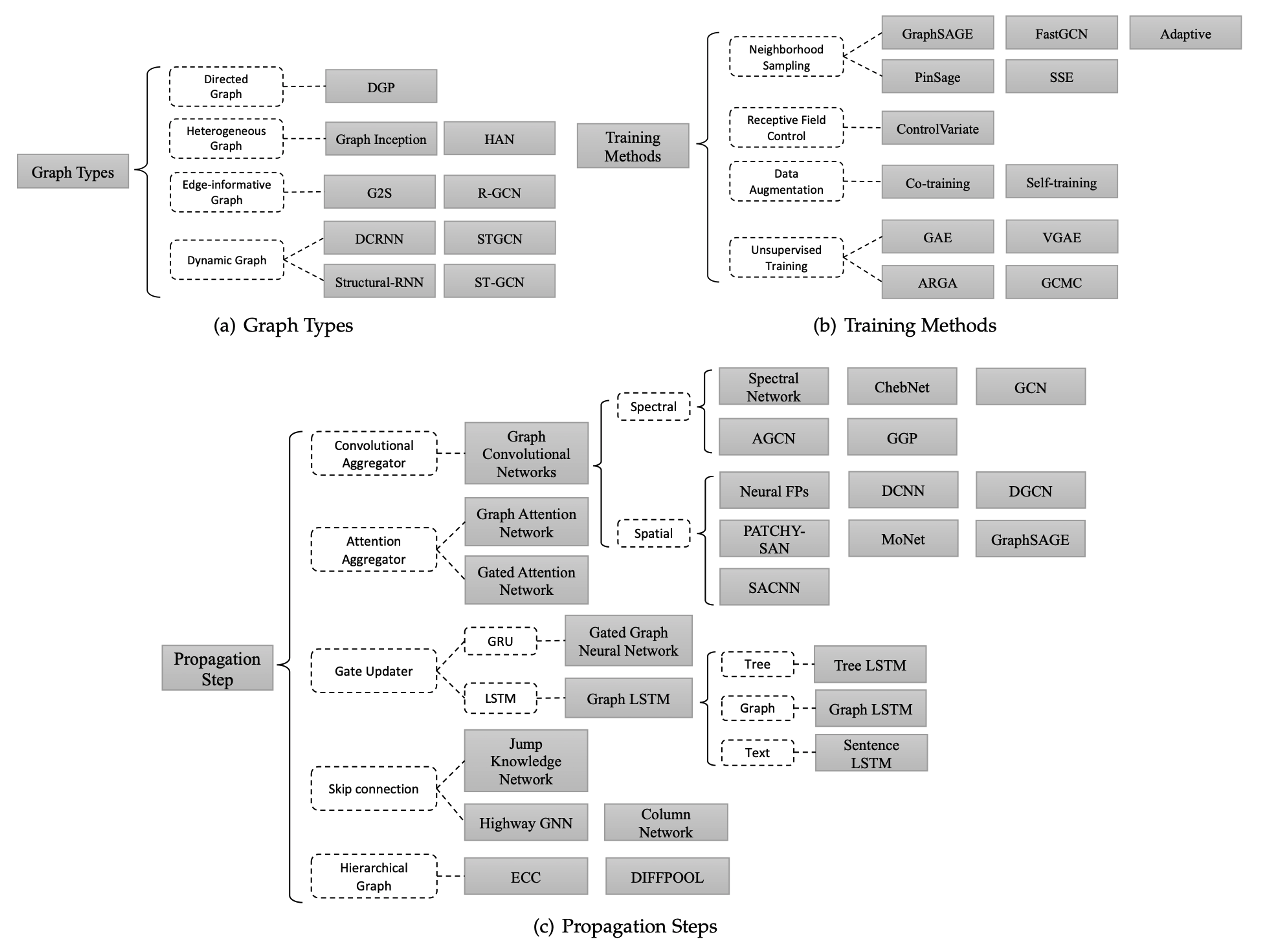
\includegraphics[width=1\textwidth]{image/gnn_1.png}
  \caption{图网络知识脉络图}
\end{figure}

\subsection{必读论文}
\begin{itemize}
    \item Ng, A. Y., Jordan, M. I., \& Weiss, Y. (2002). On spectral clustering: Analysis and an algorithm. In Advances in neural information processing systems (pp. 849-856). \\
 	吴恩达老师引用量第二的文章,谱聚类的代表作。 
 	\item Shuman, D. I., Narang, S. K., Frossard, P., Ortega, A., \& Vandergheynst, P. (2013). The emerging field of signal processing on graphs: Extending high-dimensional data analysis to networks and other irregular domains. IEEE signal processing magazine, 30(3), 83-98. \\
 	图信号处理的基本方法,算是基础。
 	\item Defferrard, M., Bresson, X., \& Vandergheynst, P. (2016). Convolutional neural networks on graphs with fast localized spectral filtering. In Advances in neural information processing systems (pp. 3844-3852). \\
 	ChebNet,图网络中频域卷积的代表作。
 	\item Kipf, T. N., \& Welling, M. (2016). Semi-supervised classification with graph convolutional networks. arXiv preprint arXiv:1609.02907. \\
 	GCN的原始论文,对ChebNet做了简化和修改。
 	\item Hamilton, W., Ying, Z., \& Leskovec, J. (2017). Inductive representation learning on large graphs. In Advances in neural information processing systems (pp. 1024-1034). \\
 	GraphSage,针对GCN只能处理固定图的缺陷,提出了一种归纳(inductive)学习的方法,使模型可以处理没有见过的节点。
 	\item Veličković, P., Cucurull, G., Casanova, A., Romero, A., Lio, P., \& Bengio, Y. (2017). Graph attention networks. arXiv preprint arXiv:1710.10903. \\
 	GAT,图上的注意力机制。
 	\item Chami, I., Ying, Z., Ré, C., \& Leskovec, J. (2019). Hyperbolic graph convolutional neural networks. In Advances in neural information processing systems (pp. 4868-4879). \\
 	在双曲空间中做图嵌入。
\end{itemize}

\section{强化学习}

\begin{figure}[htbp]
  \centering
  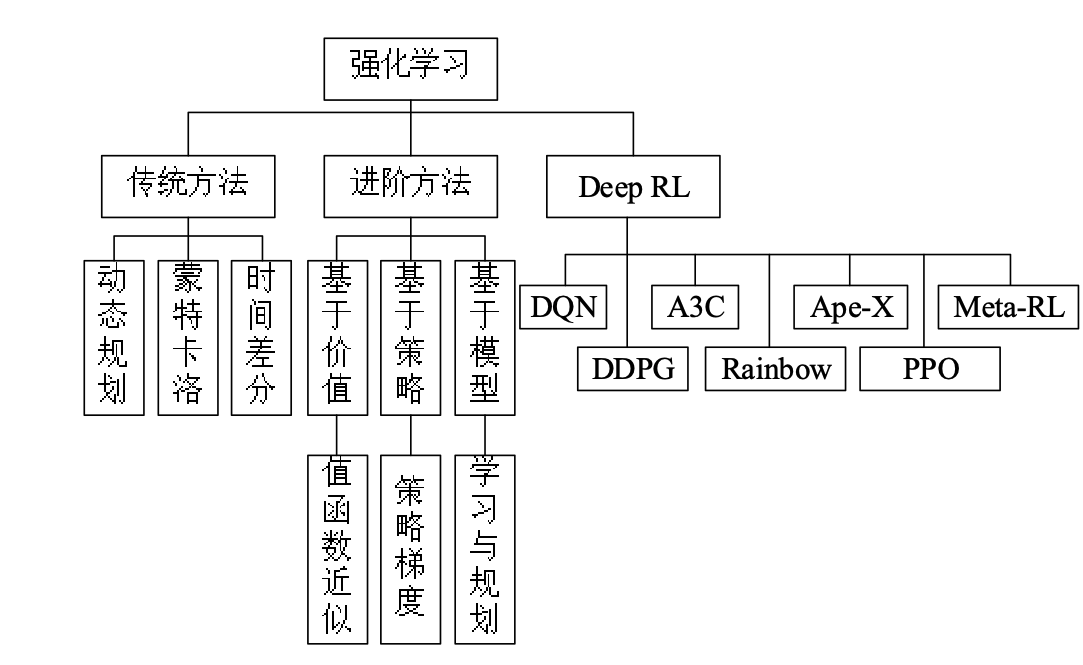
\includegraphics[width=1\textwidth]{image/rl_1.png}
  \caption{强化学习知识脉络图}
\end{figure}
学习路径:马尔科夫过程->贝尔曼方程->动态规划法->蒙特卡洛法->时间差分法->Sarsa算法->Q-learning算法->值函数近似法->策略梯度法->基于模型的强化学习->蒙特卡洛树搜索->DQN->DDPG->A3C->Rainbow->Ape-X->PPO->Meta-RL

\subsection{网课}
\begin{enumerate}
    \item 强化学习论文解读-10 mins paper,上海交大伯禹讲论文 \\
    B站伯禹账号:\href{https://space.bilibili.com/447303411}{https://space.bilibili.com/447303411}  \\
    DQN: \href{https://www.bilibili.com/video/BV1H4411d7Mh}{https://www.bilibili.com/video/BV1H4411d7Mh}  \\
    DDPG: \href{https://www.bilibili.com/video/BV18E411f7zd}{https://www.bilibili.com/video/BV18E411f7zd}  \\
    TD3: \href{https://www.bilibili.com/video/BV1nE41117CR}{https://www.bilibili.com/video/BV1nE41117CR}  \\
    PPO: \href{https://www.bilibili.com/video/BV1pE41117zu}{https://www.bilibili.com/video/BV1pE41117zu}  \\
    Soft Actor-Critic: \href{https://www.bilibili.com/video/BV1pE41117q1}{https://www.bilibili.com/video/BV1pE41117q1}  \\
    QMIX: \href{https://www.bilibili.com/video/BV1pE411176N}{https://www.bilibili.com/video/BV1pE411176N}  \\
    VDRL: \href{https://www.bilibili.com/video/BV1nE41117qu}{https://www.bilibili.com/video/BV1nE41117qu}  \\
    Nash Q-Learning: \href{https://www.bilibili.com/video/BV1mE411b7fW}{https://www.bilibili.com/video/BV1mE411b7fW}  \\
    RL with Deep Energy-Based Policies: \href{https://www.bilibili.com/video/BV1pE41117C2}{https://www.bilibili.com/video/BV1pE41117C2}  \\
    Interactive Teaching Algorithm for IRL: \href{https://www.bilibili.com/video/BV1mE411b7eu}{ https://www.bilibili.com/video/BV1mE411b7eu} \\
    Least-Squares Temporal Difference Learning: \href{https://www.bilibili.com/video/BV1nE41117C8}{https://www.bilibili.com/video/BV1nE41117C8}
    \item 强化学习 Reinforcement Learning (莫烦 Python 教程) \\
    链接:\href{https://www.bilibili.com/video/av16921335?from=search&seid=7037144790835305588}{https://www.bilibili.com/video/av16921335?from=search\&seid=7037144790835305588} \\
    代码:\href{https://github.com/AndyYue1893/Reinforcement-learning-with-tensorflow}{https://github.com/AndyYue1893/Reinforcement-learning-with-tensorflow}  
    \item DeepMind - David Silver - UCL深度强化学习课程(2015) \\
    链接:\href{https://www.bilibili.com/video/av45357759?from=search&seid=7037144790835305588}{https://www.bilibili.com/video/av45357759?from=search\&seid=7037144790835305588}  \\
    PPT地址:\href{https://blog.csdn.net/u_say2what/article/details/89216190}{https://blog.csdn.net/u\_say2what/article/details/89216190} \\
    笔记及代码:\href{https://zhuanlan.zhihu.com/p/37690204}{https://zhuanlan.zhihu.com/p/37690204} 
    \item 台大李宏毅 深度强化学习(国语)课程(2018) \\
    链接:\href{https://www.bilibili.com/video/av24724071?from=search&seid=7037144790835305588}{https://www.bilibili.com/video/av24724071?from=search\&seid=7037144790835305588}  \\
    PPT地址:\href{https://www.bilibili.com/video/av24724071?from=search&seid=7037144790835305588}{https://www.bilibili.com/video/av24724071?from=search\&seid=7037144790835305588}  \\
    学习笔记:\href{https://blog.csdn.net/cindy_1102/article/details/87904928}{https://blog.csdn.net/cindy\_1102/article/details/87904928} 
    \item UC Berkeley - Sergey Levine - CS285(294)深度强化学习(2019) \\
    链接:\href{https://www.bilibili.com/video/av69455099?from=search&seid=7037144790835305588}{https://www.bilibili.com/video/av69455099?from=search\&seid=7037144790835305588}  \\
    PPT地址:\href{http://rail.eecs.berkeley.edu/deeprlcourse/}{http://rail.eecs.berkeley.edu/deeprlcourse/}  \\
    代码:\href{https://github.com/berkeleydeeprlcourse/homework}{https://github.com/berkeleydeeprlcourse/homework}
\end{enumerate}

\subsection{书籍}
\begin{enumerate}
    \item 强化学习(第2版)(Rich Sutton)\\ 链接:\href{https://item.jd.com/12696004.html}{https://item.jd.com/12696004.html} \\
    介绍:基础必读,有助于理解强化学习精髓 \\
    英文电子版:\href{http://incompleteideas.net/book/the-book-2nd.html}{http://incompleteideas.net/book/the-book-2nd.html}  \\
    代码:\href{https://github.com/AndyYue1893/reinforcement-learning-an-introduction}{https://github.com/AndyYue1893/reinforcement-learning-an-introduction}  
    \item Python强化学习实战:应用OpenAI Gym和TensorFlow精通强化学习和深度强化学习(Sudharsan.Ravichandiran)\\
    链接:\href{https://item.jd.com/12506442.html}{https://item.jd.com/12506442.html}  \\
    代码:\href{https://github.com/AndyYue1893/Hands-On-Reinforcement-Learning-With-Python}{https://github.com/AndyYue1893/Hands-On-Reinforcement-Learning-With-Python} 
    \item 强化学习精要:核心算法与TensorFlow实现(冯超)\\
    链接:\href{https://item.jd.com/12344157.html}{https://item.jd.com/12344157.html}  \\
    代码:\href{https://pan.baidu.com/share/init?surl=nQpNbhkI-3WucSD0Mk7Qcg}{https://pan.baidu.com/share/init?surl=nQpNbhkI-3WucSD0Mk7Qcg} 提取码: av5p
    \item 深度强化学习原理与实践(陈仲铭)\\
    链接:\href{https://item.jd.com/12524381.html}{https://item.jd.com/12524381.html} \\
    代码:\href{https://github.com/chenzomi12/Deep-Reinforcement-Learning}{https://github.com/chenzomi12/Deep-Reinforcement-Learning} 
\end{enumerate}

\subsection{经典论文}
\subsubsection{典型应用}
\begin{enumerate}
    \item AlphaGo:\href{https://www.nature.com/articles/nature16961}{https://www.nature.com/articles/nature16961},战胜人类棋手,David Silver等人发表于Nature
    \item 玩Atari:\href{https://deepmind.com/research/publications/playing-atari-deep-reinforcement-learning}{https://deepmind.com/research/publications/playing-atari-deep-reinforcement-learning},游戏领域超过普通玩家
    \item 玩Pong:\href{http://karpathy.github.io/2016/05/31/rl/}{http://karpathy.github.io/2016/05/31/rl/} 
    \item 教小人走路:\href{https://arxiv.org/abs/1707.02286}{https://arxiv.org/abs/1707.02286},Deepmind出品,入门必玩项目
    \item 控制机械臂:\href{https://ai.googleblog.com/2016/03/deep-learningfor-robots-learningfrom.html}{https://ai.googleblog.com/2016/03/deep-learningfor-robots-learningfrom.html}
\end{enumerate}

\subsubsection{传统方法}
\begin{enumerate}
    \item 蒙特卡洛估计:\\
    \href{https://link.springer.com/chapter/10.1007/11871842_29}{https://link.springer.com/chapter/10.1007/11871842\_29}
    \item 时间差分学习:\\
    \href{https://www.researchgate.net/publication/2371944_Off-Policy_Temporal-Difference_Learning_with_Function_Approximation}{Off-Policy Temporal-Difference Learning with Function Approximation}
\end{enumerate}

\subsubsection{强化学习理论}
\begin{enumerate}
    \item Policy Gradient Methods for Reinforcement Learning with Function Approximation \\
    链接:\href{https://papers.nips.cc/paper/1713-policy-gradient-methods-for-reinforcement-learning-with-function-approximation.pdf}{https://papers.nips.cc/paper/1713-policy-gradient-methods-for-reinforcement-learning-with-function-approximation.pdf}, Sutton et al, 2000. \\
    主要贡献: 建立policy gradient理论,并展示出对任意policy classes,算法都可以收敛。
    \item An Analysis of Temporal-Difference Learning with Function Approximation \\
    链接:\href{http://web.mit.edu/jnt/www/Papers/J063-97-bvr-td.pdf}{http://web.mit.edu/jnt/www/Papers/J063-97-bvr-td.pdf}, Tsitsiklis and Van Roy, 1997. \\
    主要贡献: RL中价值学习方法的各种收敛结果和反例。
    \item Reinforcement Learning of Motor Skills with Policy Gradients \\
    链接:\href{http://www.kyb.mpg.de/fileadmin/user_upload/files/publications/attachments/Neural-Netw-2008-21-682_48670.pdf}{http://www.kyb.mpg.de/fileadmin/user\_upload/files/publications/attachments/Neural-Netw-2008-21-682\_48670.pdf}, Peters and Schaal, 2008. \\
    主要贡献:彻底地回顾了当时policy gradient各种方法,其中有很多现在依然是非常有用的DRL方法。
    \item Approximately Optimal Approximate Reinforcement Learning \\
    链接:\href{https://people.eecs.berkeley.edu/~pabbeel/cs287-fa09/readings/KakadeLangford-icml2002.pdf}{https://people.eecs.berkeley.edu/~pabbeel/cs287-fa09/readings/KakadeLangford-icml2002.pdf}, Kakade and Langford, 2002. \\
    主要贡献:单调优化理论的早期来源,是后来TRPO和其他算法的理论依据。
    \item A Natural Policy Gradient  \\
    链接:\href{https://papers.nips.cc/paper/2073-a-natural-policy-gradient.pdf}{https://papers.nips.cc/paper/2073-a-natural-policy-gradient.pdf}, Kakade, 2002. \\
    主要贡献:在RL中引入了natural gradients,后来在deep RL中引入了TRPO、ACKTR和其他一些方法。
    \item Algorithms for Reinforcement Learning  \\
    链接:\href{https://sites.ualberta.ca/~szepesva/papers/RLAlgsInMDPs.pdf}{https://sites.ualberta.ca/~szepesva/papers/RLAlgsInMDPs.pdf}, Szepesvari, 2009. \\
    主要贡献:在DRL之前对RL的基础和理论背景进行了综合讲解
\end{enumerate}

\subsubsection{Model-Free RL} 
\paragraph{a. Deep Q-Learning}
\begin{enumerate}
    \item Playing Atari with Deep Reinforcement Learning:\\ \href{https://www.cs.toronto.edu/~vmnih/docs/dqn.pdf}{https://www.cs.toronto.edu/~vmnih/docs/dqn.pdf}, Mnih et al, 2013. \textbf{Algorithm: DQN.}
    \item Deep Recurrent Q-Learning for Partially Observable MDPs:\\ \href{https://arxiv.org/abs/1507.06527}{https://arxiv.org/abs/1507.06527}, Hausknecht and Stone, 2015. \textbf{Algorithm: Deep Recurrent Q-Learning.}
    \item Dueling Network Architectures for Deep Reinforcement Learning:\\ \href{https://arxiv.org/abs/1511.06581}{https://arxiv.org/abs/1511.06581}, Wang et al, 2015. \textbf{Algorithm: Dueling DQN.}
    \item Deep Reinforcement Learning with Double Q-learning:\\ \href{https://arxiv.org/abs/1509.06461}{https://arxiv.org/abs/1509.06461}, Hasselt et al 2015. \textbf{Algorithm: Double DQN.}
    \item Prioritized Experience Replay:\\ \href{https://arxiv.org/abs/1511.05952}{https://arxiv.org/abs/1511.05952}, Schaul et al, 2015. \textbf{Algorithm: Prioritized Experience Replay (PER).}
    \item Rainbow: Combining Improvements in Deep Reinforcement Learning:\\ \href{https://arxiv.org/abs/1710.02298}{https://arxiv.org/abs/1710.02298}, Hessel et al, 2017. \textbf{Algorithm: Rainbow DQN.}
\end{enumerate}

\paragraph{b. Policy Gradients}
\begin{enumerate}
    \item Asynchronous Methods for Deep Reinforcement Learning:\\ \href{https://arxiv.org/abs/1602.01783}{https://arxiv.org/abs/1602.01783}, Mnih et al, 2016. \textbf{Algorithm: A3C.}
    \item Trust Region Policy Optimization:\\ \href{https://arxiv.org/abs/1502.05477}{https://arxiv.org/abs/1502.05477}, Schulman et al, 2015. \textbf{Algorithm: TRPO.}
    \item High-Dimensional Continuous Control Using Generalized Advantage Estimation:\\ \href{https://arxiv.org/abs/1506.02438}{https://arxiv.org/abs/1506.02438}, Schulman et al, 2015. \textbf{Algorithm: GAE.}
    \item Proximal Policy Optimization Algorithms:\\ \href{https://arxiv.org/abs/1707.06347}{https://arxiv.org/abs/1707.06347}, Schulman et al, 2017. \textbf{Algorithm: PPO-Clip, PPO-Penalty.}
    \item Emergence of Locomotion Behaviours in Rich Environments:\\ \href{https://arxiv.org/abs/1707.02286}{https://arxiv.org/abs/1707.02286}, Heess et al, 2017. \textbf{Algorithm: PPO-Penalty.}
    \item Scalable trust-region method for deep reinforcement learning using Kronecker-factored approximation:\\ \href{https://arxiv.org/abs/1708.05144}{https://arxiv.org/abs/1708.05144}, Wu et al, 2017. \textbf{Algorithm: ACKTR.}
    \item Sample Efficient Actor-Critic with Experience Replay:\\ \href{https://arxiv.org/abs/1611.01224}{https://arxiv.org/abs/1611.01224}, Wang et al, 2016. \textbf{Algorithm: ACER.}
    \item Soft Actor-Critic: Off-Policy Maximum Entropy Deep Reinforcement Learning with a Stochastic Actor:\\ \href{https://arxiv.org/abs/1801.01290}{https://arxiv.org/abs/1801.01290}, Haarnoja et al, 2018. \textbf{Algorithm: SAC.}
\end{enumerate}

\paragraph{c. Deterministic Policy Gradients}
\begin{enumerate}
    \item Deterministic Policy Gradient Algorithms:\\ \href{http://proceedings.mlr.press/v32/silver14.pdf}{http://proceedings.mlr.press/v32/silver14.pdf}, Silver et al, 2014. \textbf{Algorithm: DPG.}
    \item Continuous Control With Deep Reinforcement Learning:\\ \href{https://arxiv.org/abs/1509.02971}{https://arxiv.org/abs/1509.02971}, Lillicrap et al, 2015. \textbf{Algorithm: DDPG.}
    \item Addressing Function Approximation Error in Actor-Critic Methods:\\ \href{https://arxiv.org/abs/1802.09477}{https://arxiv.org/abs/1802.09477}, Fujimoto et al, 2018. \textbf{Algorithm: TD3.}
\end{enumerate}

\paragraph{d. Distributional RL}
\begin{enumerate}
    \item A Distributional Perspective on Reinforcement Learning:\\ \href{https://arxiv.org/abs/1707.06887}{https://arxiv.org/abs/1707.06887}, Bellemare et al, 2017. \textbf{Algorithm: C51.}
    \item Distributional Reinforcement Learning with Quantile Regression:\\ \href{https://arxiv.org/abs/1710.10044}{https://arxiv.org/abs/1710.10044}, Dabney et al, 2017. \textbf{Algorithm: QR-DQN.}
    \item Implicit Quantile Networks for Distributional Reinforcement Learning:\\ \href{https://arxiv.org/abs/1806.06923}{https://arxiv.org/abs/1806.06923}, Dabney et al, 2018. \textbf{Algorithm: IQN.}
    \item Dopamine: A Research Framework for Deep Reinforcement Learning:\\ \href{https://openreview.net/forum?id=ByG_3s09KX}{https://openreview.net/forum?id=ByG\_3s09KX}, Anonymous, 2018. \textbf{Contribution:} 介绍了Dopamine, 一个实现了DQN, C51, IQN, 和Rainbow等算法的代码仓. [Code link.
\end{enumerate}

\paragraph{e. Policy Gradients with Action-Dependent Baselines}
\begin{enumerate}
    \item Q-Prop: Sample-Efficient Policy Gradient with An Off-Policy Critic:\\ \href{https://arxiv.org/abs/1611.02247}{https://arxiv.org/abs/1611.02247}, Gu et al, 2016. \textbf{Algorithm: Q-Prop.}
    \item Action-depedent Control Variates for Policy Optimization via Stein’s Identity:\\ \href{https://arxiv.org/abs/1710.11198}{https://arxiv.org/abs/1710.11198}, Liu et al, 2017. \textbf{Algorithm: Stein Control Variates.}
    \item The Mirage of Action-Dependent Baselines in Reinforcement Learning:\\ \href{https://arxiv.org/abs/1802.10031}{https://arxiv.org/abs/1802.10031}, Tucker et al, 2018. \textbf{Contribution:} 这篇论文中,对以前的论文中的说法(包括Q-Prop和Stein Control Variates)进行了批判和重新评价,并发现其中存在重要的方法论错误。
\end{enumerate}

\paragraph{f. Path-Consistency Learning}
\begin{enumerate}
    \item Bridging the Gap Between Value and Policy Based Reinforcement Learning:\\ \href{https://arxiv.org/abs/1702.08892}{https://arxiv.org/abs/1702.08892}, Nachum et al, 2017. \textbf{Algorithm: PCL.}
    \item Trust-PCL: An Off-Policy Trust Region Method for Continuous Control:\\ \href{https://arxiv.org/abs/1707.01891}{https://arxiv.org/abs/1707.01891}, Nachum et al, 2017. \textbf{Algorithm: Trust-PCL.}
\end{enumerate}

\paragraph{g. Other Directions for Combining Policy-Learning and Q-Learning}
\begin{enumerate}
    \item Combining Policy Gradient and Q-learning:\\ \href{https://arxiv.org/abs/1611.01626}{https://arxiv.org/abs/1611.01626}, O’Donoghue et al, 2016. \textbf{Algorithm: PGQL.}
    \item The Reactor: A Fast and Sample-Efficient Actor-Critic Agent for Reinforcement Learning:\\ \href{https://arxiv.org/abs/1704.04651}{https://arxiv.org/abs/1704.04651}, Gruslys et al, 2017. \textbf{Algorithm: Reactor.}
    \item Interpolated Policy Gradient: Merging On-Policy and Off-Policy Gradient Estimation for Deep Reinforcement Learning:\\ \href{http://papers.nips.cc/paper/6974-interpolated-policy-gradient-merging-on-policy-and-off-policy-gradient-estimation-for-deep-reinforcement-learning}{http://papers.nips.cc/paper/6974-interpolated-policy-gradient-merging-on-policy-and-off-policy-gradient-estimation-for-deep-reinforcement-learning}, Gu et al, 2017. \textbf{Algorithm: IPG.}
    \item Equivalence Between Policy Gradients and Soft Q-Learning:\\ \href{https://arxiv.org/abs/1704.06440}{https://arxiv.org/abs/1704.06440}, Schulman et al, 2017. \textbf{Contribution:} 揭示了这两类RL算法之间的理论联系。
\end{enumerate}

\paragraph{h. Evolutionary Algorithms}
\begin{enumerate}
    \item Evolution Strategies as a Scalable Alternative to Reinforcement Learning:\\ \href{https://arxiv.org/abs/1703.03864}{https://arxiv.org/abs/1703.03864}, Salimans et al, 2017. \textbf{Algorithm: ES.}
\end{enumerate}

\subsubsection{Model-Based RL}
\paragraph{a. Model is Learned}
\begin{enumerate}
    \item Imagination-Augmented Agents for Deep Reinforcement Learning:\\ \href{https://arxiv.org/abs/1707.06203}{https://arxiv.org/abs/1707.06203}, Weber et al, 2017. \textbf{Algorithm: I2A.}
    \item Neural Network Dynamics for Model-Based Deep Reinforcement Learning with Model-Free Fine-Tuning:\\ \href{https://arxiv.org/abs/1708.02596}{https://arxiv.org/abs/1708.02596}, Nagabandi et al, 2017. \textbf{Algorithm: MBMF.}
    \item Model-Based Value Expansion for Efficient Model-Free Reinforcement Learning:\\ \href{https://arxiv.org/abs/1803.00101}{https://arxiv.org/abs/1803.00101}, Feinberg et al, 2018. \textbf{Algorithm: MVE.}
    \item Sample-Efficient Reinforcement Learning with Stochastic Ensemble Value Expansion:\\ \href{https://arxiv.org/abs/1807.01675}{https://arxiv.org/abs/1807.01675}, Buckman et al, 2018. \textbf{Algorithm: STEVE.}
    \item Model-Ensemble Trust-Region Policy Optimization:\\ \href{https://openreview.net/forum?id=SJJinbWRZ&noteId=SJJinbWRZ}{https://openreview.net/forum?id=SJJinbWRZ\&noteId=SJJinbWRZ}, Kurutach et al, 2018. \textbf{Algorithm: ME-TRPO.}
    \item Model-Based Reinforcement Learning via Meta-Policy Optimization:\\ \href{https://arxiv.org/abs/1809.05214}{https://arxiv.org/abs/1809.05214}, Clavera et al, 2018. \textbf{Algorithm: MB-MPO.}
    \item Recurrent World Models Facilitate Policy Evolution:\\ \href{https://arxiv.org/abs/1809.01999}{https://arxiv.org/abs/1809.01999}, Ha and Schmidhuber, 2018.
\end{enumerate}


\paragraph{b. Model is Given}
\begin{enumerate}
    \item Mastering Chess and Shogi by Self-Play with a General Reinforcement Learning Algorithm:\\ \href{https://arxiv.org/abs/1712.01815}{https://arxiv.org/abs/1712.01815}, Silver et al, 2017. \textbf{Algorithm: AlphaZero.}
    \item Thinking Fast and Slow with Deep Learning and Tree Search:\\ \href{https://arxiv.org/abs/1705.08439}{https://arxiv.org/abs/1705.08439}, Anthony et al, 2017. \textbf{Algorithm: ExIt.}
\end{enumerate}


\subsubsection{Imitation Learning \& Inverse Reinforcement Learning}
\begin{enumerate}
    \item Guided Cost Learning: Deep Inverse Optimal Control via Policy Optimization:\\ \href{https://arxiv.org/abs/1603.00448}{https://arxiv.org/abs/1603.00448}, Finn et al, 2016. \textbf{Algorithm: GCL.}
    \item Maximum Entropy Deep Inverse Reinforcement Learning:\\ \href{http://arxiv.org/abs/1507.04888}{http://arxiv.org/abs/1507.04888}, M. Wulfmeier et al., *arXiv*, 2015.
    \item Modeling Purposeful Adaptive Behavior with the Principle of Maximum Causal Entropy:\\ \href{http://www.cs.cmu.edu/~bziebart/publications/thesis-bziebart.pdf}{http://www.cs.cmu.edu/~bziebart/publications/thesis-bziebart.pdf}, Ziebart 2010. \textbf{Contributions:} 最大熵IRL的公式提出和推导.
    \item Generative Adversarial Imitation Learning:\\ \href{https://arxiv.org/abs/1606.03476}{https://arxiv.org/abs/1606.03476}, Ho and Ermon, 2016. \textbf{Algorithm: GAIL.}
    \item DeepMimic: Example-Guided Deep Reinforcement Learning of Physics-Based Character Skills:\\ \href{https://xbpeng.github.io/projects/DeepMimic/2018_TOG_DeepMimic.pdf}{https://xbpeng.github.io/projects/DeepMimic/2018\_TOG\_DeepMimic.pdf}, Peng et al, 2018. \textbf{Algorithm: DeepMimic.}
    \item Variational Discriminator Bottleneck: Improving Imitation Learning, Inverse RL, and GANs by Constraining Information Flow:\\ \href{https://arxiv.org/abs/1810.00821}{https://arxiv.org/abs/1810.00821}, Peng et al, 2018. \textbf{Algorithm: VAIL.}
    \item One-Shot High-Fidelity Imitation: Training Large-Scale Deep Nets with RL:\\ \href{https://arxiv.org/abs/1810.05017}{https://arxiv.org/abs/1810.05017}, Le Paine et al, 2018. \textbf{Algorithm: MetaMimic.}
\end{enumerate}

\subsubsection{Multi-Task and Transfer Learning}
\begin{enumerate}
    \item Actor-Mimic: Deep Multitask and Transfer Reinforcement Learning:\\ \href{http://arxiv.org/abs/1511.06342}{http://arxiv.org/abs/1511.06342}, E. Parisotto, et al., *ICLR*, 2016.
    \item Policy Distillation:\\ \href{http://arxiv.org/abs/1511.06295}{http://arxiv.org/abs/1511.06295}, A. A. Rusu et at., *ICLR*, 2016.
    \item ADAAPT: A Deep Architecture for Adaptive Policy Transfer from Multiple Sources:\\ \href{http://arxiv.org/abs/1510.02879}{http://arxiv.org/abs/1510.02879}, J. Rajendran et al., *arXiv*, 2015.
    \item Universal Value Function Approximators:\\ \href{http://schaul.site44.com/publications/uvfa.pdf}{http://schaul.site44.com/publications/uvfa.pdf}, T. Schaul et al., *ICML*, 2015.\textbf{Algorithm: UVFA.}
    \item Progressive Neural Networks:\\ \href{https://arxiv.org/abs/1606.04671}{https://arxiv.org/abs/1606.04671}, Rusu et al, 2016. \textbf{Algorithm: Progressive Networks.}
    \item Reinforcement Learning with Unsupervised Auxiliary Tasks:\\ \href{https://arxiv.org/abs/1611.05397}{https://arxiv.org/abs/1611.05397}, Jaderberg et al, 2016. \textbf{Algorithm: UNREAL.}
    \item The Intentional Unintentional Agent: Learning to Solve Many Continuous Control Tasks Simultaneously:\\ \href{https://arxiv.org/abs/1707.03300}{https://arxiv.org/abs/1707.03300}, Cabi et al, 2017. \textbf{Algorithm: IU Agent.}
    \item PathNet: Evolution Channels Gradient Descent in Super Neural Networks:\\ \href{https://arxiv.org/abs/1701.08734}{https://arxiv.org/abs/1701.08734}, Fernando et al, 2017. \textbf{Algorithm: PathNet.}
    \item Mutual Alignment Transfer Learning:\\ \href{https://arxiv.org/abs/1707.07907}{https://arxiv.org/abs/1707.07907}, Wulfmeier et al, 2017. \textbf{Algorithm: MATL.}
    \item Learning an Embedding Space for Transferable Robot Skills:\\ \href{https://openreview.net/forum?id=rk07ZXZRb&noteId=rk07ZXZRb}{https://openreview.net/forum?id=rk07ZXZRb\&noteId=rk07ZXZRb}, Hausman et al, 2018.
    \item Hindsight Experience Replay:\\ \href{https://arxiv.org/abs/1707.01495}{https://arxiv.org/abs/1707.01495}, Andrychowicz et al, 2017. \textbf{Algorithm: Hindsight Experience Replay (HER).}
\end{enumerate}

\subsubsection{Meta-RL}
\begin{enumerate}
    \item RL\^2: Fast Reinforcement Learning via Slow Reinforcement Learning:\\ \href{https://arxiv.org/abs/1611.02779}{https://arxiv.org/abs/1611.02779}, Duan et al, 2016. \textbf{Algorithm: RL\^2.}
    \item Learning to Reinforcement Learn:\\ \href{https://arxiv.org/abs/1611.05763}{https://arxiv.org/abs/1611.05763}, Wang et al, 2016.
    \item Model-Agnostic Meta-Learning for Fast Adaptation of Deep Networks:\\ \href{https://arxiv.org/abs/1703.03400}{https://arxiv.org/abs/1703.03400}, Finn et al, 2017. \textbf{Algorithm: MAML.}
    \item A Simple Neural Attentive Meta-Learner:\\ \href{https://openreview.net/forum?id=B1DmUzWAW&noteId=B1DmUzWAW}{https://openreview.net/forum?id=B1DmUzWAW\&noteId=B1DmUzWAW}, Mishra et al, 2018. \textbf{Algorithm: SNAIL.}
\end{enumerate}

\subsubsection{Improving Exploration}
\paragraph{a. Intrinsic Motivation}
\begin{enumerate}
    \item VIME: Variational Information Maximizing Exploration:\\ \href{https://arxiv.org/abs/1605.09674}{https://arxiv.org/abs/1605.09674}, Houthooft et al, 2016. \textbf{Algorithm: VIME.}
    \item Unifying Count-Based Exploration and Intrinsic Motivation:\\ \href{https://arxiv.org/abs/1606.01868}{https://arxiv.org/abs/1606.01868}, Bellemare et al, 2016. \textbf{Algorithm: CTS-based Pseudocounts.}
    \item Count-Based Exploration with Neural Density Models:\\ \href{https://arxiv.org/abs/1703.01310}{https://arxiv.org/abs/1703.01310}, Ostrovski et al, 2017. \textbf{Algorithm: PixelCNN-based Pseudocounts.}
    \item \#Exploration: A Study of Count-Based Exploration for Deep Reinforcement Learning:\\ \href{https://arxiv.org/abs/1611.04717}{https://arxiv.org/abs/1611.04717}, Tang et al, 2016. \textbf{Algorithm: Hash-based Counts.}
    \item EX2: Exploration with Exemplar Models for Deep Reinforcement Learning:\\ \href{https://arxiv.org/abs/1703.01260}{https://arxiv.org/abs/1703.01260}, Fu et al, 2017. \textbf{Algorithm: EX2.}
    \item Curiosity-driven Exploration by Self-supervised Prediction:\\ \href{https://arxiv.org/abs/1705.05363}{https://arxiv.org/abs/1705.05363}, Pathak et al, 2017. \textbf{Algorithm: Intrinsic Curiosity Module (ICM).}
    \item Large-Scale Study of Curiosity-Driven Learning:\\ \href{https://arxiv.org/abs/1808.04355}{https://arxiv.org/abs/1808.04355}, Burda et al, 2018. \textbf{Contribution:} 系统分析基于好奇心的内在动机算法在各种环境中的表现
    \item Exploration by Random Network Distillation:\\ \href{https://arxiv.org/abs/1810.12894}{https://arxiv.org/abs/1810.12894}, Burda et al, 2018. \textbf{Algorithm: RND.}
\end{enumerate}

\paragraph{b. Unsupervised RL}
\begin{enumerate}
    \item Variational Intrinsic Control:\\ \href{https://arxiv.org/abs/1611.07507}{https://arxiv.org/abs/1611.07507}, Gregor et al, 2016. \textbf{Algorithm: VIC.}
    \item Diversity is All You Need: Learning Skills without a Reward Function:\\ \href{https://arxiv.org/abs/1802.06070}{https://arxiv.org/abs/1802.06070}, Eysenbach et al, 2018. \textbf{Algorithm: DIAYN.}
    \item Variational Option Discovery Algorithms:\\ \href{https://arxiv.org/abs/1807.10299}{https://arxiv.org/abs/1807.10299}, Achiam et al, 2018. \textbf{Algorithm: VALOR.}
\end{enumerate}

\subsubsection{Multi-Agent}
\begin{enumerate}
    \item Learning to Communicate to Solve Riddles with Deep Distributed Recurrent Q-Networks:\\ \href{http://arxiv.org/abs/1602.02672}{http://arxiv.org/abs/1602.02672}, J. N. Foerster et al., *arXiv*, 2016.
    \item Multiagent Cooperation and Competition with Deep Reinforcement Learning:\\ \href{http://arxiv.org/abs/1511.08779}{http://arxiv.org/abs/1511.08779}, A. Tampuu et al., *arXiv*, 2015.
\end{enumerate}

\subsubsection{Hierarchical Learning}
\begin{enumerate}
    \item Deep Successor Reinforcement Learning:\\ \href{http://arxiv.org/abs/1606.02396}{http://arxiv.org/abs/1606.02396}, T. D. Kulkarni et al., *arXiv*, 2016.
    \item Hierarchical Reinforcement Learning using Spatio-Temporal Abstractions and Deep Neural Networks:\\ \href{https://arxiv.org/abs/1605.05359}{https://arxiv.org/abs/1605.05359}, R. Krishnamurthy et al., *arXiv*, 2016.
    \item Hierarchical Deep Reinforcement Learning: Integrating Temporal Abstraction and Intrinsic Motivation:\\ \href{https://arxiv.org/abs/1604.06057}{https://arxiv.org/abs/1604.06057}, T. D. Kulkarni et al., *arXiv*, 2016.
    \item Strategic Attentive Writer for Learning Macro-Actions:\\ \href{https://arxiv.org/abs/1606.04695}{https://arxiv.org/abs/1606.04695}, Vezhnevets et al, 2016. \textbf{Algorithm: STRAW.}
    \item FeUdal Networks for Hierarchical Reinforcement Learning:\\ \href{https://arxiv.org/abs/1703.01161}{https://arxiv.org/abs/1703.01161}, Vezhnevets et al, 2017. \textbf{Algorithm: Feudal Networks}
    \item Data-Efficient Hierarchical Reinforcement Learning:\\ \href{https://arxiv.org/abs/1805.08296}{https://arxiv.org/abs/1805.08296}, Nachum et al, 2018. \textbf{Algorithm: HIRO.}
\end{enumerate}

\subsubsection{Safety}
\begin{enumerate}
    \item Concrete Problems in AI Safety:\\ \href{https://arxiv.org/abs/1606.06565}{https://arxiv.org/abs/1606.06565}, Amodei et al, 2016. \textbf{Contribution:} 建立安全问题的分类,这个方向需要解决的问题。
    \item Deep Reinforcement Learning From Human Preferences:\\ \href{https://arxiv.org/abs/1706.03741}{https://arxiv.org/abs/1706.03741}, Christiano et al, 2017. \textbf{Algorithm: LFP.}
    \item Constrained Policy Optimization:\\ \href{https://arxiv.org/abs/1705.10528}{https://arxiv.org/abs/1705.10528}, Achiam et al, 2017. \textbf{Algorithm: CPO.}
    \item Safe Exploration in Continuous Action Spaces:\\ \href{https://arxiv.org/abs/1801.08757}{https://arxiv.org/abs/1801.08757}, Dalal et al, 2018. \textbf{Algorithm: DDPG+Safety Layer.}
    \item Trial without Error: Towards Safe Reinforcement Learning via Human Intervention:\\ \href{https://arxiv.org/abs/1707.05173}{https://arxiv.org/abs/1707.05173}, Saunders et al, 2017. \textbf{Algorithm: HIRL.}
    \item Leave No Trace: Learning to Reset for Safe and Autonomous Reinforcement Learning:\\ \href{https://arxiv.org/abs/1711.06782}{https://arxiv.org/abs/1711.06782}, Eysenbach et al, 2017. \textbf{Algorithm: Leave No Trace.}
\end{enumerate}

\subsubsection{Memory}
\begin{enumerate}
    \item Model-Free Episodic Control:\\ \href{https://arxiv.org/abs/1606.04460}{https://arxiv.org/abs/1606.04460}, Blundell et al, 2016. \textbf{Algorithm: MFEC.}
    \item Neural Episodic Control:\\ \href{https://arxiv.org/abs/1703.01988}{https://arxiv.org/abs/1703.01988}, Pritzel et al, 2017. \textbf{Algorithm: NEC.}
    \item Neural Map: Structured Memory for Deep Reinforcement Learning:\\ \href{https://arxiv.org/abs/1702.08360}{https://arxiv.org/abs/1702.08360}, Parisotto and Salakhutdinov, 2017. \textbf{Algorithm: Neural Map.}
    \item Unsupervised Predictive Memory in a Goal-Directed Agent:\\ \href{https://arxiv.org/abs/1803.10760}{https://arxiv.org/abs/1803.10760}, \\ Wayne et al, 2018. \textbf{Algorithm: MERLIN.}
    \item Relational Recurrent Neural Networks:\\ \href{https://arxiv.org/abs/1806.01822}{https://arxiv.org/abs/1806.01822}, Santoro et al, 2018. \textbf{Algorithm: RMC.}
\end{enumerate}

\subsubsection{Scaling RL(分布式RL)}
\begin{enumerate}
\item Accelerated Methods for Deep Reinforcement Learning:\\ \href{https://arxiv.org/abs/1803.02811}{https://arxiv.org/abs/1803.02811}, Stooke and Abbeel, 2018. \textbf{Contribution:} 跨算法的深度RL中的并行化系统分析。
\item IMPALA: Scalable Distributed Deep-RL with Importance Weighted Actor-Learner Architectures:\\ \href{https://arxiv.org/abs/1802.01561}{https://arxiv.org/abs/1802.01561}, Espeholt et al, 2018. \textbf{Algorithm: IMPALA.}
\item Distributed Prioritized Experience Replay:\\ \href{https://openreview.net/forum?id=H1Dy---0Z}{https://openreview.net/forum?id=H1Dy---0Z}, Horgan et al, 2018. \textbf{Algorithm: Ape-X.}
\item Recurrent Experience Replay in Distributed Reinforcement Learning:\\ \href{https://openreview.net/forum?id=r1lyTjAqYX}{https://openreview.net/forum?id=r1lyTjAqYX}, Anonymous, 2018. \textbf{Algorithm: R2D2.}
\item RLlib: Abstractions for Distributed Reinforcement Learning:\\ \href{https://arxiv.org/abs/1712.09381}{https://arxiv.org/abs/1712.09381}, Liang et al, 2017. \textbf{Contribution:} 提出一个实现了17年前大部分RL算法的可扩展库。
\end{enumerate}


\subsubsection{RL in the Real World}
\begin{enumerate}
\item Benchmarking Reinforcement Learning Algorithms on Real-World Robots:\\ \href{https://arxiv.org/abs/1809.07731}{https://arxiv.org/abs/1809.07731}, Mahmood et al, 2018.
\item Learning Dexterous In-Hand Manipulation:\\ \href{https://arxiv.org/abs/1808.00177}{https://arxiv.org/abs/1808.00177}, OpenAI, 2018.
\item QT-Opt: Scalable Deep Reinforcement Learning for Vision-Based Robotic Manipulation:\\ \href{https://arxiv.org/abs/1806.10293}{https://arxiv.org/abs/1806.10293}, Kalashnikov et al, 2018. \textbf{Algorithm: QT-Opt.}
\item Horizon: Facebook’s Open Source Applied Reinforcement Learning Platform:\\ \href{https://arxiv.org/abs/1811.00260}{https://arxiv.org/abs/1811.00260}, Gauci et al, 2018.
\end{enumerate}

\subsubsection{RL的可复现性等方面的分析} 
\begin{enumerate}
\item Benchmarking Deep Reinforcement Learning for Continuous Control:\\ \href{https://arxiv.org/abs/1604.06778}{https://arxiv.org/abs/1604.06778}, Duan et al, 2016. \textbf{Contribution: rllab库.}
\item Reproducibility of Benchmarked Deep Reinforcement Learning Tasks for Continuous Control:\\ \href{https://arxiv.org/abs/1708.04133}{https://arxiv.org/abs/1708.04133}, Islam et al, 2017.
\item Deep Reinforcement Learning that Matters:\\ \href{https://arxiv.org/abs/1709.06560}{https://arxiv.org/abs/1709.06560}, Henderson et al, 2017.
\item Where Did My Optimum Go?: An Empirical Analysis of Gradient Descent Optimization in Policy Gradient Methods:\\ \href{https://arxiv.org/abs/1810.02525}{https://arxiv.org/abs/1810.02525}, Henderson et al, 2018.
\item Are Deep Policy Gradient Algorithms Truly Policy Gradient Algorithms?:\\ \href{https://arxiv.org/abs/1811.02553}{https://arxiv.org/abs/1811.02553}, Ilyas et al, 2018.
\item Simple Random Search Provides a Competitive Approach to Reinforcement Learning:\\ \href{https://arxiv.org/abs/1803.07055}{https://arxiv.org/abs/1803.07055}, Mania et al, 2018.
\item Benchmarking Model-Based Reinforcement Learning:\\ \href{https://arxiv.org/abs/1907.02057}{https://arxiv.org/abs/1907.02057}, Wang et al, 2019.
\end{enumerate}




\end{document}
\end{lstlisting}

\nocite{*}

\end{document}
